\makeatletter
%\newcommand{\rmnum}[1]{\romannumeral #1 }
%\newcommand{\Rmnum}[1]{\expandafter\@slowromancap\romannumeral #1@}
\makeatother
\ifpdf
\graphicspath{{Chapter1/Chapter1Figs/PNG/}{Chapter1/Chapter1Figs/PDF/}{Chapter1/Chapter1Figs/}}
\else
\graphicspath{{Chapter1/Chapter1Figs/EPS/}{Chapter1/Chapter1Figs/}}
\fi

\chapter{BERI Coherence Models}
\label{chapter_coherence}

In this chapter I introduce the BERI cache coherence protocols. I discuss the architectural details of both designs, including all optimisations added through evaluations in simulation and FPGA hardware. The parallel performance of the coherence protocols is presented in Chapter \ref{coherence_eval}.

The BERI directory-based coherence scheme uses a full directory approach. It tracks private sharer caches through a shared last level cache. This coherence scheme complies with the TSO memory consistency model, typically used on x86 systems.

The BERI time-based coherence protocol, assigns a timestamp to every cached line. This allows the protocol to forego coherence messaging. It uses standard memory communication to fetch data whenever an expired cache line is accessed. This protocol requires the appropriate usage of software synchronisation and locking instructions. 
However, no dedicated software support is necessary as barriers and locks are widely used by software.

A well defined memory consistency model is critical to provide software assurances. The time-based coherence scheme supports RMO memory consistency, specifically RMO{\large$^\star$} (defined in Section \ref{background_consistency}). The compliance of this cache coherence scheme is thoroughly verified through memory consistency checking tools presented in Chapter \ref{chapter_validation}. 

A relaxed memory consistency model may offer some parallel performance advantages, however, the main reason for selecting this model is that it simplifies the hardware design constraints and eliminates the need for any explicit coherence messaging. Additionally, it is widely supported by popular operating systems such as FreeBSD, and compilers such as LLVM. This memory model is also used in commercial architectures such as ARM and PowerPC. In its current form, the time-based coherence protocol cannot support a stronger coherence model, but stronger support is typically unnecessary.


\clearpage
\section{BERI Time-Based Coherence}
	\label{section_timebased_coherence}
	Communication centric cache coherence protocols focus on a bottom up approach, maintaining and distributing coherence information through the last-level cache (LLC) or a dedicated memory controller.
	The time-based coherence model goes against this principle by controlling coherence from within the private caches.
	In the absence of explicit coherence messaging, cache flushing is one way of updating stale data and restoring system coherence. 
	Behavioural correctness of the time-based coherence model relies on implementation elements such as the cache self-invalidation technique, explicit synchronisation instructions, and lock-free atomic instructions. 

	Software data structures are often stored contiguously in memory, and repeated data operations can be significantly sped-up through caching. Thus, choosing an appropriate cache line lifespan in a time-based coherence cache is non trivial. There is a constant tradeoff between miss rates due to counter overflows and the cache capacity overheads. In order to retain the benefits of data caching, the lifespan of each line must be long enough to maintain a low miss rate, as well as short enough to allow timely stale data eviction. This coherence model does not directly expose cache line time-outs, so software must use correct locking structures and barriers to ensure appropriate data sharing.

	\subsection{Time Counter}
		In the current BERI multiprocessor implementation, each L1 data cache has a dedicated time-counter. This counter governs the cache self-invalidation policy. The time-counter increments are dictated by the cache cycle counter and the synchronisation (SYNC) instruction. 
		The maximum tick range of the cycle counter can be selected during hardware synthesis and currently is not modifiable through software.
		
		Every time-counter tick can be referred to as the time-out, since all cache lines loaded prior to the tick become invalid.
		Figure \ref{beri_timebased_algorithm} illustrates this behaviour.
		A full cache flush is triggered when the time-counter rolls over, this is done using the cache initialisation logic, all memory access to the cache are blocked during this flush. Frequent counter roll-overs may result in a slow cache response time, so there is a tradeoff between the counter size and cache storage overheads. 

	\subsection{Tag Timestamp}
		Each L1 data cache line contains data bits and tag bits, stored in separate memory blocks. A timestamp is added to the tag bits, this tag-time-stamp (TTS) dictates the cache line lifespan. TTS is set when a line is cached for the first time, this value is generated by adding 1 to the current time-counter.
		When a cache line is requested and it is a hit, the TTS is compared to the current time-counter value. Line lifespan expires when the time-counter is greater than TTS, this forces a cache miss. A valid TTS allows the cache to proceed as normal.

		\begin{figure}[t]
			\centering 
				\makebox{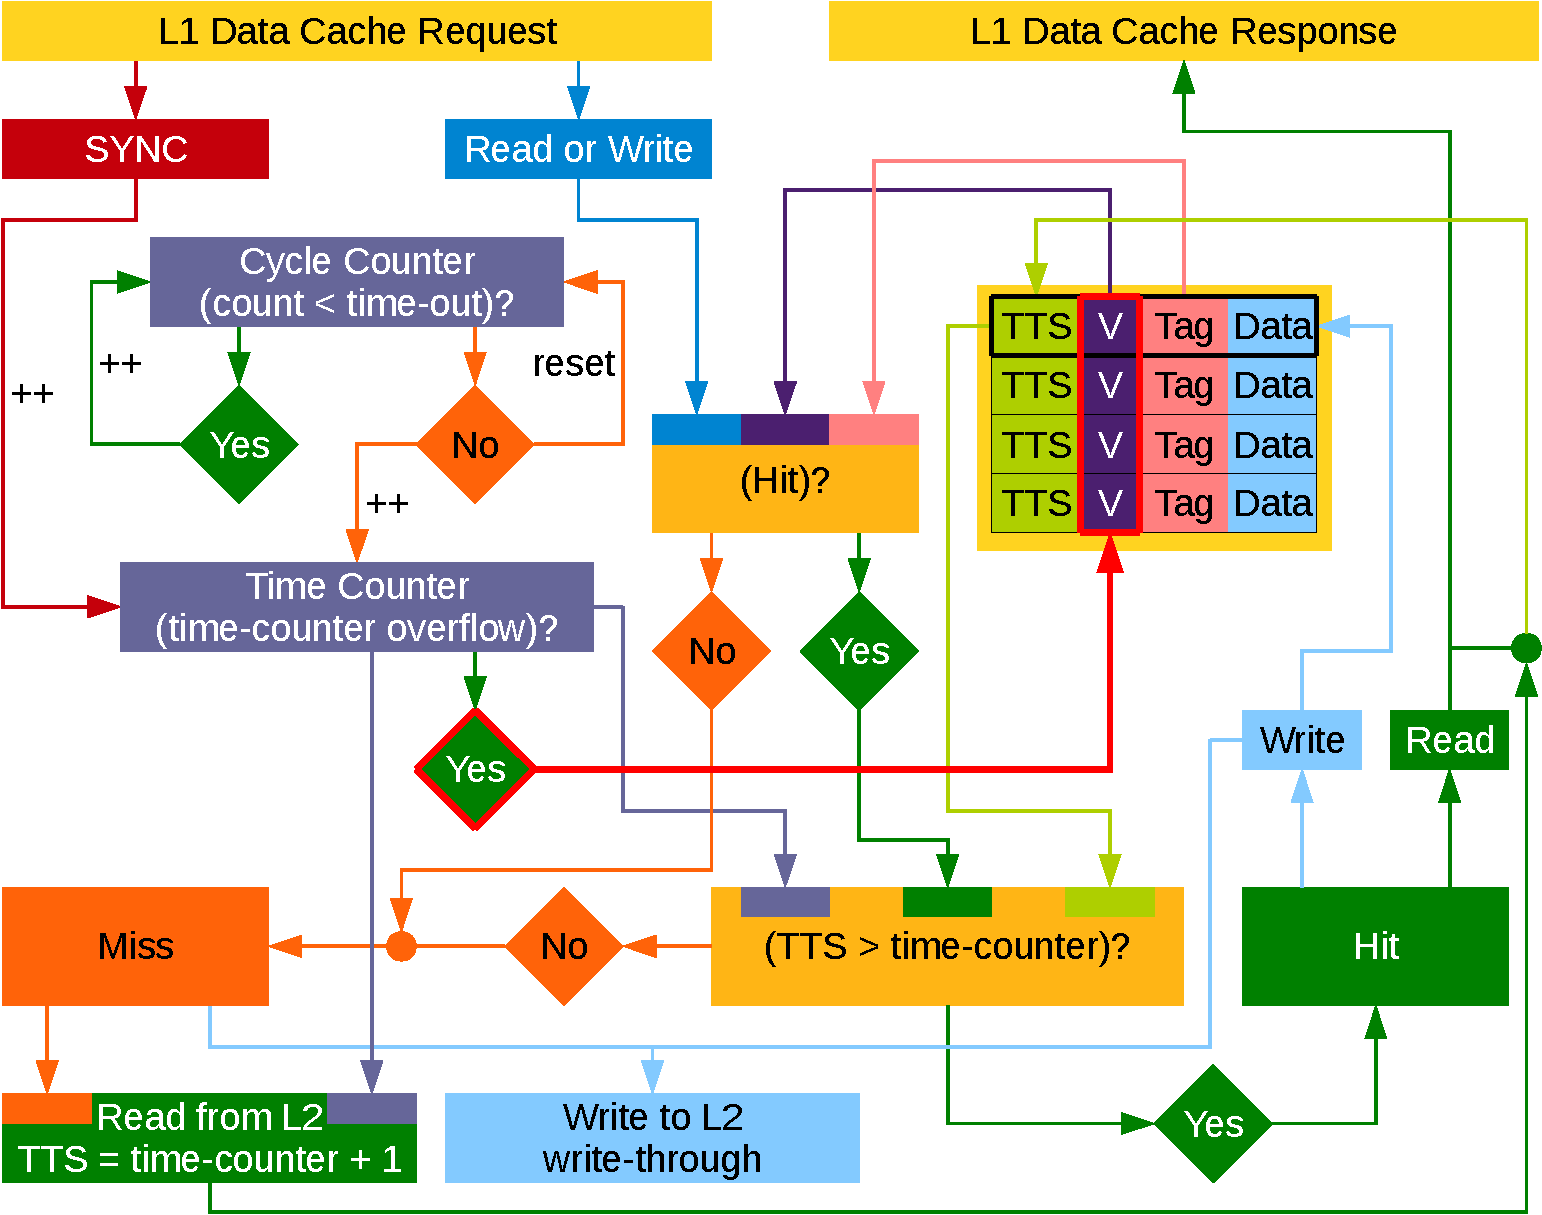
\includegraphics[width=\textwidth,height=\textheight,keepaspectratio]{BERI_timebased_algorithm}}
				\caption[BERI time-based coherence mechanism]{BERI time-based coherence mechanism (L1 data cache)} 
				\label{beri_timebased_algorithm}
		\end{figure}
	
	\subsection{Time-out Selection}
		Time tick granularity used for self-invalidation is dictated by the cycle counter. It can be varied from a single cycle to infinity. In the evaluation chapter we will see how the choice of cache line time-outs affects system performance. Its easy to assume that long time-outs will keep data cached and benefit overall performance, however, holding on to shared data and waiting for SYNCs does not fit all software behaviour. 		
		The performance of software relying on polling operations may suffer due to infrequent data updates. Polling operations rely on updates to memory locations and may not use any SYNC instructions, hence, time-outs are necessary. 
		
		Eliminating cache time-outs may result in unpredictable OS behaviour, an increased likelihood of deadlocks, and an overall performance drop. 
		The time-out procedure ensures some progress, regardless of other synchronisation operations. However, waiting for a time-out could cause lengthy delays. Some memory polling patterns can be detected by hardware.
		
		Software relying on lock-free atomic instructions is not affected by time-outs; on multi-core BERI these instructions bypass local caches. They are frequently used for synchronisation. Additionally, a generous use of SYNCs in FreeBSD allows time-based coherence to function correctly. FreeBSD synchronisation and locking statistics are detailed in Chapter \ref{coherence_eval}, coherence results and evaluation. Deadlock avoidance is discussed in Section \ref{litmus_perfromance}.

	\subsection{Polling Detection Mechanism}
		\label{polling_detection_mechanism}
		This L1 cache based mechanism eliminates one of the major drawbacks of time-based coherence; slow updates to polled memory locations, caused by stale data caching and a potentially large cycle delay between self-invalidates. OS schedulers may use memory polling as a part of the scheduling mechanism. The access patterns can be predicted in hardware, leading to a reduction in memory overheads. The OS polling behaviour and profiling techniques are illustrated by Frigui and Alfa \cite{Frigui95}.  Further motivations and design choices of the BERI polling optimisation are explained in Section \ref{sync_only_coherence}, SYNC-only coherence. 

		\begin{figure}[!t]
		\begin{tcolorbox}[
		colback=cyan!1!white,
		colframe=cyan!75!black]
\begin{center}
\begin{BVerbatim}
if (read hit)  // query polling table
	if (valid && address match)
		delete table entry;
		force read miss;
	else
		return data;
if (write hit) // query polling table
	if (valid && address match)
		delete table entry;
		write-through data;
	else
		write local data;
		write-through data;	
if (read miss) // fetch data from L2
	if (empty polling table entry)
		add new address;
	else
		delete random entry;
		add new address;
	return data;
if (write miss) // non write allocate
	write-through data;
\end{BVerbatim}
\end{center}		
		\end{tcolorbox}
		\caption{L1 data cache memory polling detector}
		\label{polling_detector_diagram}
		\end{figure}

		The detector tracks cache load misses. When the data is fetched, it saves the physical addresses into a 4 register fully associative lookup table. 
		The physical address of each new cache load request is compared against valid entries in the detector lookup table. 
		An address match indicates that the requested memory location has not been locally updated since it was first loaded. 
		This behaviour is typically exhibited by a memory polling operation. 
		When such a memory location is identified, a miss is forced by the detector and an updated value is fetched from shared memory. 
		The pseudocode for this algorithm is presented in Figure \ref{polling_detector_diagram}.
		
		Table entries are deleted whenever a store matches one of the entries. A random replacement policy is used whenever the table runs of empty memory slots. Based on FreeBSD observations, a 4 entry table should be sufficient. 
		However, some software behaviour may be different, and more table entries or an alternative detection technique may be necessary.
		In the event of a polling misprediction, the time-based automatic self-invalidation mechanism ensures that stale data will be eventually updated and some progress will be made.
		
		Time-based coherence benefits from this mechanism, as it significantly speeds up synchronisation through polling.
		The algorithm is independent of the coherence model and could be added to other schemes.
		However, designs such as the directory approach are unlikely to benefit from polling detection, since the coherence scheme itself ensures stale data eviction.
		Furthermore, false polling detection is likely to cause a performance degradation.
	

	\subsection{TTS Memory Overhead}
		\label{tts_memory_overhead}
		There is a tradeoff between the time-counter register size and the penalty for counter roll-overs. A smaller time-counter size increases the frequency of roll-overs, leading to frequent full cache flushes. Note that time-counter size is independent of the number of cycles per time-counter tick. 
		Darnell and Kennedy \cite{Darnell93} have shown that cache line timestamps as low as 1 bit can be used. However, their scheme relies on explicit software epochs aimed at select memory locations. The SYNC instruction has a similar effect in the BERI time-based scheme, but the cache can also automatically self-invalidate lines. 
		
		In more recent work by Elver and Nagarajan \cite{Elver14}, 4 bit timestamps are added to memory locations, reducing the sharer tracking overheads of MESI coherence (Chapter \ref{chapter_background}). I have opted to use a 4 bit TTS size, as the storage overheads for two L1 data caches (2$_{cores}$$\times$4$_{bits}$$\times$512$_{l1-lines}$ = 4096) is identical to the directory overhead in the L2 cache (2$_{cores}$$\times$1$_{bit/core}$$\times$2048$_{l2-lines}$ = 4096). Figures \ref{dcache_tags_short_tts} and \ref{big_dcache_tags_short_tts} compare tag overheads with increasing cache capacity (tags have been padded to 32 bits in order to simplify the visual comparison). 
		
		The counter size must be carefully considered when synthesising these caches on an FPGA, as block RAM (BRAM) design will greatly affect optimisation. The tag size tradeoff is also critical, when a certain size is exceeded, multiple BRAM's may be necessary. ASIC designs are more flexible, as arbitrarily sized tags, data lines, and other components can be produced.

		\begin{figure}[t]
		\centering
			\newcommand{\colorbitbox}[3]{%
			\rlap{\bitbox{#2}{\color{#1}\rule{\width}{\height}}}%
			\bitbox{#2}{#3}}
			\definecolor{lightcyan}{rgb}{0.6,1,1}
			\definecolor{lightgreen}{rgb}{0.7,1,0.7}
			\definecolor{lightred}{rgb}{1,0.7,0.7}
			\definecolor{lightgray}{gray}{0.8}
			\begin{bytefield}[bitheight=\widthof{~Valid~},bitwidth=\widthof{\large x~},
			boxformatting={\centering\small}]{32}
			\bitheader[endianness=big]{31,30,27,26,25,0} \\
			\bitbox{1}{\color{lightgray}\rule{\width}{\height}} &
			\colorbitbox{lightgreen}{4}{TTS} &
			\colorbitbox{lightcyan}{1}{\rotatebox{90}{Valid}} &
			\colorbitbox{lightred}{26}{Tag}
			\end{bytefield}
			\caption[L1 data cache tags, 16KB cache]{L1 data cache tags, 4 bit TTS (16KB cache size)} \label{dcache_tags_short_tts}
		\vspace{5mm}

			\centering	
			\begin{bytefield}[bitheight=\widthof{~Valid~},bitwidth=\widthof{\large x~},
			boxformatting={\centering\small}]{32}
			\bitheader[endianness=big]{31,30,29,26,25,24,0} \\
			\bitbox{2}{\color{lightgray}\rule{\width}{\height}} &
			\colorbitbox{lightgreen}{4}{TTS} &
			\colorbitbox{lightcyan}{1}{\rotatebox{90}{Valid}} &
			\colorbitbox{lightred}{25}{Tag}
			\end{bytefield}
			\caption[L1 data cache tags, 32KB cache]{L1 data cache tags, 4 bit TTS (32KB cache size)} \label{big_dcache_tags_short_tts}
		\end{figure}
		
		Our RISC processor only requires 40 bits of physical address space. When the cache size is increased, fewer tag bits are required since fewer address bits are stored in the tags. Figure \ref{big_dcache_tags_short_tts} shows this effect when the cache size is doubled. 
		One additional bit will be used for cache indexing, so the tag is shrunk. This can be beneficial for time-based coherence, since a larger TTS can be used without increasing the relative storage overheads.
		
		The time-based coherence model does not add any overheads to the L2 cache and the LL/SC mechanism is identical to the one used by BERI directory coherence. The L2 cache tag structure for the time-based coherence mechanism and the LL/SC overheads are discussed in Section \ref{dir_llc_structure}, and compared against the directory-based coherence model.
		
	\subsection{SYNC Instruction Behaviour}
		\label{sync_behaviour}
		This instruction performs two operations in the L1 data cache. 
		Firstly, the time-counter is incremented on SYNC (Figure \ref{beri_sync}), ensuring that all stale data will be treated as invalid, it can also be interpreted as a single instruction full cache flush. 
		Note that if the SYNC instruction causes the time-counter to overflow, then the cache is reinitialised. 
		
		The second property of this instruction is to ensure that all loads/stores have been propagated to the LLC. 
		This is achieved by performing a flush to LLC, this memory access has no side-effects. The operation blocks the cache until a response is received. The response guarantees load/store propagation from the given core. The response is ignored by the pipeline as SYNC instructions are not expected to respond. 
		The SYNC mechanism used in the directory coherence model is also shown in Figure \ref{beri_sync} for a direct comparison. Since the directory does not use time-counters, the SYNC instruction simply ensures that all memory operations have propagated to the shared cache.
		
		Instruction caches do not self-invalidate; coherence is not necessary for instructions as long as self-modifying code is not executed.
		
		\begin{figure}[t]
			\centering 
				\makebox{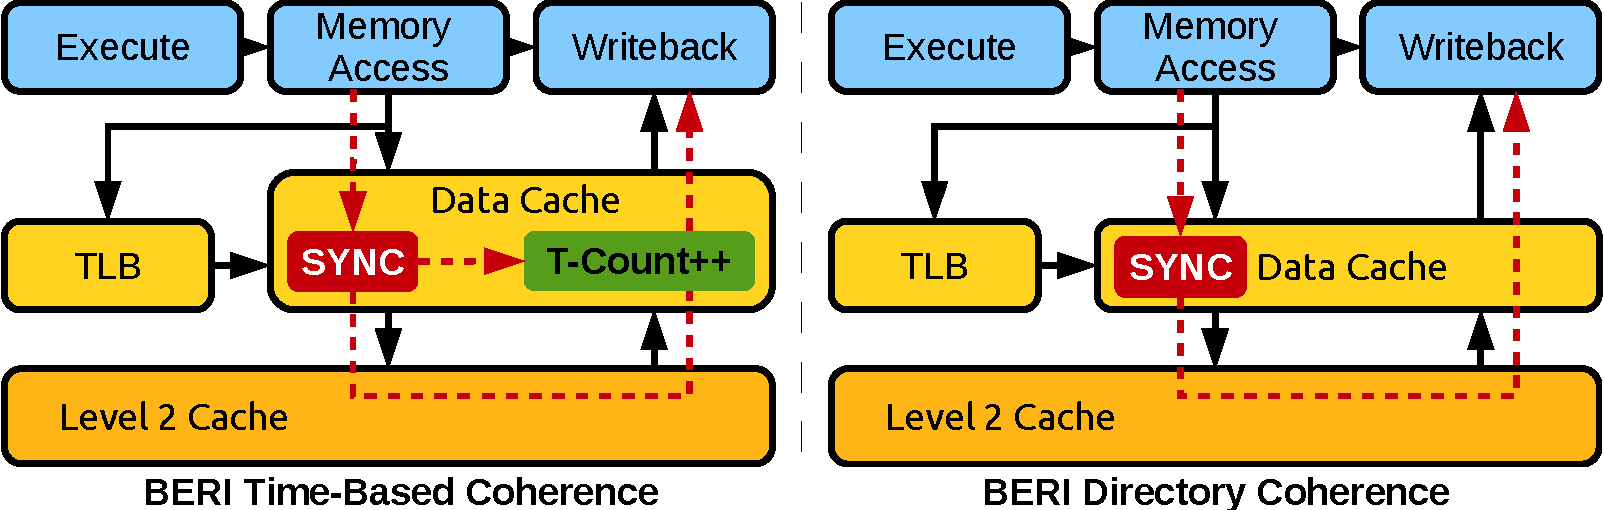
\includegraphics[width=\textwidth,height=\textheight,keepaspectratio]{BERI_sync}}
				\caption{BERI multiprocessor SYNC mechanism} 
				\label{beri_sync}
		\end{figure}


%\clearpage
\subsection{SYNC-only Coherence}
	\label{sync_only_coherence}
	
	%TODO: cost per invalidate for directory coherence
	
	%We have established that time-based coherence presents a functional memory consistency model, usable and supported by FreeBSD. In the evaluation Chapter \ref{coherence_eval} we will see that time-based coherence tends to show better parallel performance with increasing cache line lifespan. We have also seen the effects of a SYNC instruction on the cache behaviour. 
	
	It is possible to design a coherence scheme relying solely on SYNC instructions, using neither self-invalidation or coherence messaging. However, a few potential limitations include: insufficient or incorrect usage of synchronisation primitives, polling, and other schemes relying on strong hardware coherence.
	Memory polling operations can be implemented through other software primitives, without any need for special instructions. Alternatively, a hardware polling detection mechanism can be used, but it may not be able to detect and resolve all cases.
	
	For instance, on a dual-core BERI system, the FreeBSD booting mechanism uses core 0 by default. Once the initial boot set-up is complete, core 0 signals core 1 through shared memory and initiates parallel tasks. Core 1 waits for the update by running a simple loop consisting of a load instruction followed by a branch. It is easy for hardware to detect this operation as all core 1 memory accesses are loads to the same address with no local updates. The polling detector can be implemented by using a single register in each private cache to track a load to an unmodified location. One register is sufficient in this example but it may be insufficient in other scenarios.
	
	A hardware instruction trace of the FreeBSD file copy application (CP) has shown that during its execution a two stage polling operation is observed. The trace shows two loads to independent memory locations, separated by branch instructions. Software jumps between the two load operations with no other memory instruction in between. At least two polling detection registers are required to correctly identify this behaviour. 
	
	Testing on FreeBSD has not revealed polling mechanisms requiring more than two separate load addresses, such as the CP scenario. I implemented an in cache, 4 register polling detector, that complements the self-invalidation mechanism. 
	The polling detector is sufficiently wide to track most polling operations, and long delays between self-invalidations retain the hit ratios required by parallel applications. If this mechanism were to guarantee precise detection of all polling accesses, cache time-outs could be eliminated entirely and all coherence operations would be controlled through synchronisation instructions.


%\clearpage
\section{BERI Directory Coherence}
	\label{section_directory_coherence}
		The BERI multiprocessor architecture was initially designed using more conventional coherence mechanisms, unlike the time-based scheme discussed previously. The BERI directory-based design is the outcome of a refined exploration of communication centric coherence protocols.

		One of the simplest coherence protocols for a shared memory system is Invalidate On Write (IOW) \cite{Hennessy06}. Coherence is maintained by broadcasting invalidation messages whenever a store operation is performed in the shared cache. This protocol requires a cache write-through policy, since a write-back policy will allow the cache to hold dirty lines until they get evicted. Without explicit barriers or other means of data propagation, coherence will fail. The IOW coherence mechanism suffers large coherence communication overheads, since every store operation generates a broadcast message \cite{Lawrence98,Tomasevic92,Hennessy06}. 
		
		\textcolor{red}{Many have said that write-through data caches (private) are not actively used in modern CPU's, however, the recent generations of AMD processors have all relied on this cache data propagation protocol. (TODO: citation http://www.realworldtech.com/bulldozer/9/)}
		
		
		
		
		\textcolor{red}{Copy of the document starts here >>>>}
		 Since the L1D is both write-through and mostly included in the L2, evicting a cache line from the L1D is silent and requires no further actions. This is beneficial since evictions are typically caused by a filling a cache line, in response to a cache miss and closely tied to the critical path for a miss. In the exclusive L1D cache for Istanbul, moving the evicted line from L1D to L2 contributed to the latency for a cache miss.
		
		The relationship between the L1D and L2 caches also simplifies reliability. Since any data written by the L1D is also present in the L2, parity is sufficient protection for the L1; any errors can be fixed by reloading from the ECC protected L2 (or L3/memory). As a result, ECC is no longer required for the L1D (as it was for Istanbul), which reduces the power consumption for stores. In Istanbul, any store to a cache line had to first read to get the ECC, then recalculate the ECC with the new data and then finally write to the cache.
		
		While the L1D is mostly included in the L2, there are some situations where lines can reside in the L1D without being present in the L2. As a result, the L1D may need to be snooped when another core misses in the L3 cache. This is extremely undesirable, since there will be substantial snoop traffic in a Bulldozer system which will cost both power and performance if the L1D caches must always be snooped by remote cache misses. In Nehalem, the L3 cache is inclusive precisely to eliminate this sort of snoop traffic. It stands to reason that Bulldozer was designed to eliminate snoop traffic to the L1D caches and instead have the L2 cache for each module handle all the coherency snoops for that module. Unfortunately, AMD was unwilling to disclose the precise nature of their coherency protocol at Hot Chips, so we will have to wait to find out more details.
		
		One disadvantage of a write-through policy is that the L1D caches do not insulate the L2 cache from the store traffic in the cache hierarchy. Consequently, the L2 cache must have higher bandwidth to accommodate all the store traffic from two cores, and any associated snoop traffic and responses.
		
		To alleviate the write-through bandwidth requirements on the L2, each Bulldozer module includes a write coalescing cache (WCC), which is considered part of the L2. At present, AMD has not disclosed the size and associativity of the WCC, although it is probably quite small. Stores from both L1D caches go through the WCC, where they are buffered and coalesced. The purpose of the WCC is to reduce the number of writes to the L2 cache, by taking advantage of both spatial and temporal locality between stores. For example, a memcpy() routine might clear a cache line with four 128-bit stores, the WCC would coalesce these stores together and only write out once to the L2 cache.
		
		Most implementations of Bulldozer (certainly Interlagos) will share a single L3 cache, which acts as a mostly exclusive victim buffer for the L2 caches in each module. Again, AMD would not disclose any information as it concerns the overall product, rather than the core itself. However, it is possible to make an intelligent estimate based on public information. Assuming that each Interlagos die will have 8MB of L2 cache for 4 modules, the L3 is most likely to be 8MB.
		
		AMD cannot afford to produce a die with 16MB of L3 cache on 32nm and 4MB is probably too small. When Barcelona was first released on 65nm, the L3 cache was 2MB – equal to the aggregate size of the four L2 caches. It seems reasonable that AMD would return to this arrangement. The associativity is an open question, but should be at least 16-way and more likely 32 or 64 way. It is also expected that AMD has further refined and improved the sharing and contention management policies in the L3 cache.
		
		Prefetching is another area where historically Intel has relentlessly focused, and AMD has lagged behind. Prefetching can be highly effective at reducing memory latency, and can lead to tremendous increases in performance – especially for workloads with complex data structures that tend to incur many cache misses. In Bulldozer, there was a tremendous amount of effort put into the prefetching that should yield good results. The exact nature of the strided prefetchers (i.e. where addresses are offset by exactly +/-N bytes) was not discussed, but that is an area which has been very thoroughly explored in academia and commercial products.
		
		More intriguing is Bulldozer’s non-strided data prefetcher, which is useful for accessing more complex and irregular data structures (e.g. linked lists, B-trees, etc.). Again, AMD did not disclose their approach, but one possibility is what we might describe as a ‘pattern history based prefetcher’. The prefetcher tracks the addresses of misses and tries to identify specific patterns of misses that occur together (temporally). Once a pattern of misses has been detected, the prefetcher will find the first miss in the pattern. When this first miss occurs again, the prefetcher will immediately prefetch the rest of the pattern. For traversing a complex data structure like a linked list, this would be a fairly effective approach. There are other techniques that have been discussed in academic literature, and it will be interesting to see which AMD implemented.
		\textcolor{red}{Ends here <<<<}
		
		\textcolor{green}{Also see: http://www.programcreek.com/2012/12/amd-versus-intel-successes-and-pitfalls-of-their-processor-architectures-2-bulldozer-and-sandy-bridge-comparison/}
		
		\textcolor{blue}{http://delivery.acm.org/10.1145/2620000/2618129/a4-molka.pdf?ip=128.232.64.58\&id=2618129\&acc=ACTIVE\%20SERVICE\&key=BF07A2EE685417C5\%2E6CDC43D2A5950A53\%2E4D4702B0C3E38B35\%2E4D4702B0C3E38B35\&CFID=832885662\&CFTOKEN=17969456\&\_\_acm\_\_=1472754966\_7ba3a70cc008174a88a56e87443dafc2}
		%http://delivery.acm.org/10.1145/2620000/2618129/a4-molka.pdf?ip=128.232.64.58&id=2618129&acc=ACTIVE%20SERVICE&key=BF07A2EE685417C5%2E6CDC43D2A5950A53%2E4D4702B0C3E38B35%2E4D4702B0C3E38B35&CFID=832885662&CFTOKEN=17969456&__acm__=1472754966_7ba3a70cc008174a88a56e87443dafc2
		
		
		
		
		\subsection{Tracking Shared Memory}
			The IOW design was significantly improved by using a directory to accurately track all sharers of a given memory location. The directory-based protocol closely resembles the full-map directory schemes described by Hennessy and Patterson \cite{Hennessy06}, Lilja \cite{Lilja93}, and Chaiken et al. \cite{Chaiken90}. 
			
			The directory is located in the shared last level cache (LLC) and sharers are tracked by maintaining one bit per core per cache line. A combination of all shared bits for a given line is a sharers list. The list indicates whether that line is also present in one of the private caches. When the shared line receives a store operation, the sharers list identifies caches holding stale data copies. The LLC sends a coherence message to a memory controller. 
		
			The memory controller simply reads the sharers list contained within the message and then distributes invalidates to all relevant private caches. The coherence network and the memory controller are isolated from other memory communication. This allows low latency invalidate distribution. Additionally, the invalidate messages take priority over other requests in private caches. 
			
			% I-Caches
			I choose not to enforce coherence in the instruction caches, which is normally required for self-modifying code, commonly used by loaders/dynamic linkers which are capable of handling explicit software-directed instruction cache invalidation.

		\subsection{Inclusion Policy}
			Protocol correctness necessitates an accurate list of sharers, enforced through a strict cache inclusion policy. This policy indirectly affects the directory performance, since sharers must be carefully tracked and invalidated when a capacity miss is encountered. This issue is elaborated by Gupta et al. \cite{Gupta90}. 
			
			Similar to other coherence protocols requiring explicit coherence messages, the BERI directory protocol shows some communication drawbacks, not very evident with a small number of cores, but likely to escalate as the number of cores is increased in the future. 
	

		\subsection{Coherence Messaging Overheads}
			% Doesnt need ACK
			The protocol does not require coherence message acknowledgements, unlike some schemes described by Martin et al. \cite{Martin12}. This is achieved through fine tuning of coherence message delivery ensuring strong consistency compliance (TSO). Strong consistency has ensured stable FreeBSD OS support and allowed the development of the BERI multiprocessor system.
			
			Communication overheads are inevitable with a directory-based, snooping-based, or other novel communication based protocols \cite{Ros12,Hennessy06}.
			Research described in \cite{Lilja93,Sanchez12,Cuesta11,Cuesta13,James90} has shown a number of ways of optimising directory-based coherence designs through coherence message reduction, logic overheads, and understanding of sharing patterns.
			
			Relatively small scale testing of BERI has not yet necessitated these optimisations and the current protocol has been proven to work well, showing good private cache hit rates (see Chapter \ref{coherence_eval}). These characteristics provide sufficient evidence that the protocol is representative of directory-based coherence schemes and appropriate for a baseline comparison. 
		
		\subsection{Design Comparison}
			The BERI directory-coherence scheme is representative of an exact full directory mechanism. It is difficult to directly compare the BERI directory-based coherence design with other related designs, as most of the designs cannot be prototyped on the MIPS architecture without significant modifications or speculative execution. 
			
			Chapter \ref{coherence_eval} shows the performance evaluation of this protocol, the cache hit/miss ratios are comparable to non-optimised directory protocols, precision and efficiency of coherence messages is also shown. 
	
			BERI design complexity and Stratix-4 FPGA capacity currently limit the number of cores to 4. However, future design iterations and multi-FPGA interconnect could allow tens or hundreds of physical cores, necessitating a scalable coherence protocol. 
	
	\subsection{Data Cache Structure}
		\label{dir_data_cache_structure}
		The L1 data caches do not make any coherence decisions, unlike the BERI time-based model. Coherence data is supplied to the cache through a dedicated interface. The coherence message is processed by a dedicated hardware module within the cache, performing any necessary tag lookups and appropriate invalidates. Figure \ref{dir_dcache_tags} shows the tag structure for a BERI directory-based L1 data cache (tags have been padded to 32 bits in order to simplify the visual comparison). 
		
		In order to limit the side-effects of coherence messages on the general cache behaviour, an additional short-tag bank has been added. It is an optimisation and the directory scheme can be implemented without this feature. Figure \ref{dir_dcache_short_tags} shows the tag structure for an optimised directory coherence L1 data cache. The short-tag optimisation allows parallel memory access and coherence tag lookups. The short-tags are a subset of the complete physical address tag. 
		
		\begin{figure}[t]
		\centering
			\newcommand{\colorbitbox}[3]{%
			\rlap{\bitbox{#2}{\color{#1}\rule{\width}{\height}}}%
			\bitbox{#2}{#3}}
			\definecolor{lightcyan}{rgb}{0.6,1,1}
			\definecolor{lightred}{rgb}{1,0.7,0.7}
			\definecolor{lightgray}{gray}{0.8}

			\definecolor{lightorange}{rgb}{1,0.8,0.5}
			\definecolor{lightpurple}{rgb}{0.8,0.6,1}
			\definecolor{lightgreen}{rgb}{0.7,1,0.7}
			
			\definecolor{lightlightred}{rgb}{1,0.9,0.9}

			\begin{bytefield}[bitheight=\widthof{~Valid~},bitwidth=\widthof{\large x~},
			boxformatting={\centering\small}]{32}
			\bitheader[endianness=big]{31,27,26,25,0} \\
			\bitbox{5}{\color{lightgray}\rule{\width}{\height}} &
			\colorbitbox{lightcyan}{1}{\rotatebox{90}{Valid}} &
			\colorbitbox{lightred}{26}{Tag}
			\end{bytefield}
			\caption[L1 data cache tags, default]{L1 data cache tags, dual-core directory coherence (16KB cache size)} \label{dir_dcache_tags}
		\vspace{5mm}
		\centering
			\begin{bytefield}[bitheight=\widthof{~Valid~},bitwidth=\widthof{\large x~},
			boxformatting={\centering\small}]{32}
			\bitheader[endianness=big]{31,16,15,14,0} \\
			\bitbox{16}{\color{lightgray}\rule{\width}{\height}} &
			\colorbitbox{lightcyan}{1}{\rotatebox{90}{Valid}} &
			\colorbitbox{lightlightred}{15}{Short-Tag} \\
			\bitheader[endianness=big]{31,27,26,25,0} \\
			\bitbox{5}{\color{lightgray}\rule{\width}{\height}} &
			\colorbitbox{lightcyan}{1}{\rotatebox{90}{Valid}} &
			\colorbitbox{lightred}{26}{Tag}
			\end{bytefield}
			\caption[L1 data cache tags, short-tags optimisation]{L1 data cache tags, dual-core directory coherence with short-tags (16KB cache size)} \label{dir_dcache_short_tags}
		\end{figure}
		
		FPGA Block RAM's require 2 cycles to respond, one cycle to submit a BRAM request and one cycle to respond. During this operation all I/O ports of the cache are blocked. A subset of the tags is sufficient to reduce the number of false invalidates. Since parallel lookups are allowed, an invalidate operation only blocks the cache for 1 cycle instead of 2. This optimisation also helps maintaining a low coherence latency and simplifies TSO compliance. The drawbacks for using short-tags are the memory and logic overheads, however, FPGA synthesis results have not shown a significant impact in the L1 data cache size.

		An alternative to using short-tags would be either a full tag lookup or blindly invalidating cache lines. The former adds a cycle of latency and increases congestion where as the latter increases cache miss rates. As mentioned earlier, the short-tags are independently accessible and implemented in a separate BRAM. The size of the short-tags is such that for a given data cache capacity, all bits fit into a single BRAM. For this reason a total of 16 bits are used in a 16KB data cache, one valid bit and the 15 bottom bits of the physical address tag. 
		If the short-tags are valid and the select bits of the physical address match, the line will be invalidated. No action is taken otherwise. 
		
		Splash-2 Benchmarks (Chapter \ref{coherence_eval}) running on FreeBSD have shown that on an average, the short-tags optimisation offers a $\sim$2\% improvement in execution time over the full-tag version. All coherence messages issued by the directory result in some sharer cache blocking; short-tags simply reduce this penalty. This mechanism has been further analysed through memory consistency verification, bare metal tests, and correct FreeBSD behaviour. All directory-based coherence evaluation described in the dissertation uses this implementation.

		\begin{figure}[t]
		\centering
			\newcommand{\colorbitbox}[3]{%
			\rlap{\bitbox{#2}{\color{#1}\rule{\width}{\height}}}%
			\bitbox{#2}{#3}}
			\definecolor{lightcyan}{rgb}{0.6,1,1}
			\definecolor{lightred}{rgb}{1,0.7,0.7}
			\definecolor{lightgray}{gray}{0.8}

			\definecolor{lightorange}{rgb}{1,0.8,0.5}
			\definecolor{lightpurple}{rgb}{0.8,0.6,1}
			\definecolor{lightgreen}{rgb}{0.7,1,0.7}

			\begin{bytefield}[bitheight=\widthof{~Linked~},bitwidth=\widthof{\large x~},
			boxformatting={\centering\small}]{32}
			\bitheader[endianness=big]{31,28,27,26,25,24,23,0} \\
			\bitbox{4}{\color{lightgray}\rule{\width}{\height}} &
			\colorbitbox{lightpurple}{2}{\rotatebox{90}{Sharers}} &
			\colorbitbox{lightorange}{1}{\rotatebox{90}{Dirty}} &
			\colorbitbox{lightcyan}{1}{\rotatebox{90}{Valid}} &
			\colorbitbox{lightred}{24}{Tag}
			\end{bytefield}
			\caption[L2 cache tags, dual-core directory]{L2 cache tags, dual-core directory coherence (64KB cache size)} \label{dir_l2cache_tags}
		\vspace{5mm}
		\centering
			\begin{bytefield}[bitheight=\widthof{~Linked~},bitwidth=\widthof{\large x~},
			boxformatting={\centering\small}]{32}
			\bitheader[endianness=big]{31,30,29,26,25,24,23,0} \\
			\bitbox{2}{\color{lightgray}\rule{\width}{\height}} &
			\colorbitbox{lightpurple}{4}{\rotatebox{90}{Sharers}} &
			\colorbitbox{lightorange}{1}{\rotatebox{90}{Dirty}} &
			\colorbitbox{lightcyan}{1}{\rotatebox{90}{Valid}} &
			\colorbitbox{lightred}{24}{Tag}
			\end{bytefield}
			\caption[L2 cache tags, quad-core directory]{L2 cache tags, quad-core directory coherence (64KB cache size)} \label{dir_l2cache_tags_quad}
		\vspace{5mm}
		\centering
			\begin{bytefield}[bitheight=\widthof{~Linked~},bitwidth=\widthof{\large x~},
			boxformatting={\centering\small}]{32}
			\bitheader[endianness=big]{31,26,25,24,23,0} \\
			\bitbox{6}{\color{lightgray}\rule{\width}{\height}} &
			%\colorbitbox{lightpurple}{2}{\rotatebox{90}{Linked}} &
			\colorbitbox{lightorange}{1}{\rotatebox{90}{Dirty}} &
			\colorbitbox{lightcyan}{1}{\rotatebox{90}{Valid}} &
			\colorbitbox{lightred}{24}{Tag}
			\end{bytefield}
			\caption[L2 cache tags, dual-core time-based]{L2 cache tags, dual-core time-based coherence (64KB cache size)} \label{selfinv_l2_tags}
		\end{figure}

	\subsection{Last Level Cache Structure}
		\label{dir_llc_structure}
		The directory is fully contained in the LLC. Memory overheads are dramatically different between the time-based design and the directory design. The former incurs L1 data cache storage overheads, where as the latter incurs LLC storage overheads. The LLC must maintain a sharers list as specified previously. 
		
		The L2 cache overheads for the directory-based scheme are shown in Figures \ref{dir_l2cache_tags} and \ref{dir_l2cache_tags_quad} (tags have been padded to 32 bits in order to simplify the visual comparison). For comparison, the L2 cache tags for the time-based coherence model are also shown in Figure \ref{selfinv_l2_tags}. Since one bit per core is required to maintain directory coherence, the overhead is clear in Figure \ref{dir_l2cache_tags_quad}, where the costs double for a quad-core BERI. This is a typical scalability issue for a single level directory design.
		
		The shared LLC cache is write-back and maintains a fully inclusive cache policy. In order to maintain an accurate and updated sharers list, the LLC must hold copies of all the data present in the private data caches. 
		If a line is evicted from the shared cache, an invalidate must be broadcast to all sharer caches. Otherwise stale data may remain in L1 caches until the cache lines are replaced or re-fetched.
		
		The LLC cache stores tags on every memory operation. This is done to ensure that all cores accessing shared memory are included in the sharers list. 
		Failing to do so would result in inconsistencies and stale L1 data. If the OS issues a specific LLC cache invalidate instruction for a line that may be shared, all sharers of said line must be invalidated to preserve inclusion.

\clearpage
\section{Comparative Cache Design}
	\label{section_cache_properties}
	In this section I discuss how various cache design choices affect the memory coherence properties of multi-core BERI designs. The time-based model displays fewer design dependencies than the directory model, particularly when dealing with shared caches. However, it suffers a few drawbacks which are discussed below.

	\paragraph{Inclusion Policy:} This property is an attribute of a multi-tired memory hierarchy. The choice of an inclusion policy is design dependent. Maximising the total caching capacity necessitates an exclusive policy. A strictly inclusive policy requires all L1 data to be cached in lower levels as well. A non-inclusive policy permits intermediate behaviour between strictly inclusive and exclusive policies. 
	
	Shared memory communication centric coherence protocols benefit from a strictly inclusive policy, as shared memory is always aware of any privately cached data. The BERI directory model requires a strictly inclusive policy. 
	The time-based model does not require any explicit coherence messaging and any policy is acceptable. Since exclusive behaviour is not enforced, caches follow the non-inclusive policy.
	
	\paragraph{Associativity:} The storage location of a memory entry is determined by the replacement policy, ranging from direct mapped to fully associative. Maintaining coherence is simpler in direct mapped caches as all memory addresses will have a fixed location. Set associative or fully associative designs require parallel cache lookups in order to find any matching data. 
	
	Directory coherence is not directly affected by private cache associativity, however, multiple parallel coherence lookups may be necessary. Time-based coherence is not affected by associativity since coherence is only enforced during data loads or stores.
	
	\paragraph{Line Eviction:} When a cache runs out of free/invalid memory locations, the replacement policy dictates the cache line that will be replaced with new data. Direct mapped caches have a fixed policy; set associative caches can be designed with a number of cache replacement policies. The shared memory cache replacement policy will affect directory-based coherence, potentially increasing coherence messaging. Time-based coherence should not be affected, as no coherence messaging is used.
	
	\paragraph{Virtual and Physical Addressing:} Caches can be designed with various addressing modes, virtually tagged caches do not require TLB lookups where as physically tagged caches do. Coherence mechanisms benefit when shared caches and private caches use a common addressing mechanism, coherence messages are much simpler and cause fewer side-effects. All BERI caches are physically addressed, directory coherence messages carry the physical address and time-based coherence does not require messages.
	
	\paragraph{Cache Line Granularity:} BERI caches store 32 bytes of data per line. Each line shares a common valid bit and a tag field. An access miss to any word within a cache line will result in a full replacement. With the exception of aliasing which is discussed further, large lines are beneficial to both directory and time-based coherence. The memory metadata overheads are lower with a larger line size and coherence messages are more efficient as well. The tag-time-stamp used in time-based coherence has a smaller overhead as compared to a cache with a smaller line size. 
	
	\paragraph{Line Aliasing:} Mapping more than one data location to the same cache line results in aliasing. Aliasing is particularly hazardous in virtually mapped caches since two virtual addresses may point to the same physical address. Physically mapped caches are accesses through unique physical addresses, and aliasing usually results in the eviction of current cached data. Contention for the same cache line results in a degradation of performance and potential side-effects due to coherence.
	
	In coherent systems, such as the directory, memory aliasing can present a performance disadvantage. The directory must maintain an up-to-date record of any private caches sharing memory locations, when a memory line is evicted, the record must be updated as well. However, any sharers of the evicted line must be notified that the line is no longer in shared memory, failure to notify sharers will result in caching of stale data without any directory record. 
	%A strictly inclusive cache hierarchy will further exacerbate.
	
	Capacity misses in the shared cache will also result in evictions and coherence messages. This case has been observed in our directory based BERI design. The time-based coherence design is not penalised by the side-effects of aliasing memory since there is no explicit coherence messaging. Additionally this coherence model allows non-inclusive behaviour due to the absence of any sharer records. While time-based coherence has many drawbacks due to synchronisation and counter overflows, it does not suffer from aliasing overheads.
	
	\paragraph{False Sharing:} A subset of memory aliasing is false sharing of memory lines. It occurs when two memory words within a cache line are accessed independently and there is no direct data sharing. However, the coherence mechanism must keep track of any updates, particularly when the two words are accessed by different private caches. False sharing mostly results in performance degradation in the case of a directory design. As with aliasing, the time-based model is not affected by false sharing.
	
	\paragraph{Memory Operation Reordering:} Memory access reordering must behave according to a selected consistency scheme. TSO requires strict store ordering, whereas RMO permits interleaving of memory accesses. The TSO based directory coherence model must obey store ordering, necessitating precise and timely coherence messaging. The time-based coherence model uses RMO, requiring less intervention. Our cache design is fairly simple and does not offer memory access reordering within a core and its private caches, however, shared memory accesses may be out of order.
	
	\paragraph{Prefetching:} Compulsory cache misses can be reduces by fetching an entire line, when a memory word is requested. Advanced prefetchers can predict consecutive memory operations and speculatively fetch more than one line. Prefetching is beneficial for both the directory and time-based models. For both the directory and time-based design, the respective sharers list and tag-time-stamp are modified once, when the line is loaded into the cache.
	
	\paragraph{Alignment:} Any memory access that requires data between word boundaries is known as an unaligned access. Most modern systems permit unaligned accesses, the MIPS model used in BERI has a very limited support using special instructions. Since BERI does not permit accesses across cache line boundaries, we do not deal with this issue, however, as a general argument; aliment presents a challenge for both directory and time-based coherence. 
	
	The directory may require multiple sharer list accesses and the time-based model will require updating more than one TTS. Additionally a mismatched TTS may exist where one of the two lines was evicted and then reloaded. Accurate tracking of TTS entries will be necessary to avoid coherence bugs.
	
	\paragraph{Cache Instructions:} Most processors support some form of cache instructions, designed to allow cache cleaning, usually by the OS. In MIPS R4000, the cache instructions can target the L1 or the L2 caches. However, the effects of these instructions on coherence are not specified. In order to maintain the strict inclusion policy, the directory sends coherence messages to the L1 caches whenever a cache instruction evicts a shared line (applies to a single sharer scenario). Time-based coherence does not require strict inclusion, so L2 cache instructions have no effect. Respective consistency policies of the coherence schemes must also hold for cache instructions, this behaviour has been tested for both coherence models.
	
	\paragraph{Write Buffers:} Caches act as large write buffers, but many modern systems use an additional layer of buffering for improved memory accesses. Memory consistency mostly dictates the behaviour of write buffers. A TSO model requires correct write propagation through the write buffers. An RMO model allows a more relaxed behaviour, but the write buffers must propagate on synchronisation. BERI caches do not use write buffers, some buffering is present in the shared bus, but it does not affect the consistency models.
	
	\paragraph{Write Hit Policy:} There are largely two write hit policies: write-through and write-back. A write-through policy updates the current cache and propagates the update to a lower level of memory. Typically, write-back caches mark the line as dirty and hold the copy until the line is evicted or explicitly requested through coherence. BERI L1 caches are write-through. Both coherence schemes benefit from this behaviour. The write-back policy is frequently used in L1 caches, reducing memory traffic to the L2. Directory coherence requires more states to accurately track sharing patterns since writes are not immediately visible. Coherence schemes such as MESI, MOESI, MESIF, etc provide the necessary states for tracking sharing. 
	
	With write-through L1 caches, the time-based model is always guaranteed to fetch an up-to-date memory copy when a line is self-invalidated, since all stores are propagated to the L2. This approach is frequently used in related research \cite{Chen92,Choi11,Singh13,Singh14,Sung15}. 
	
	A write-back L1 will prevent the propagation of updates, but the time-based scheme can be adapted to deal with this scenario by tracking dirty lines, however, additional cache logic will be necessary. Overheads can be reduced by tracking a small number of dirty lines and periodically flushing them to the L2. This technique would allow batching of writes and reducing communication traffic, while retaining the advantages of time-based coherence. Dirty lines will need to be flushed on SYNCs, adding a performance penalty due to cache blocking during eviction. Periodic flushes and limiting the number of dirty lines may reduce this penalty.
	
	\paragraph{Write Miss Policy:} On a write miss, the cache can either request the line from a lower tier of memory and update it with new data (write allocate), or simply pass the write to a lower level of memory and leave the current cache untouched (non write allocate). BERI caches use the non write allocate policy. Directory and time-based coherence can accommodate both policies natively. A write allocate policy would perform a load from shared memory and a directory would register the requester as a sharer. The time-based model would assign a tag-time-stamp to the loaded and updated line.

\clearpage
\section{Coherence Hardware Overhead Comparison}
	\label{section_fpga_overheads}
	Coherence mechanisms typically add logic, wiring, and memory overheads. The overheads for the BERI directory and time-based coherence models are highlighted in this section. The absence of a coherence network limits the overheads of the time-based model, making it more efficient than the directory version.

	\paragraph{Time-Based Coherence Overheads}
	\begin{itemize}
	\item L1 data cache: Tag-time-counter and time-counter comparators. Polling detection logic, 4 registers each holding a physical address.
	\item Time-counter: Size of the counter is implementation dependant, in this version, 4 bits are used for the time-counter and 20 bits for the secondary cycle counter.
	\item Tag-time-counter: Every L1 data cache line requires this counter. TTS size will depend on the selection of the cache time-counter, 4 bits in this implementation (4$\times$512 bits for 16KB direct-mapped data cache, 32 bytes per line).
	\end{itemize}
	
	\paragraph{Directory Coherence Overheads}
	\begin{itemize}
	\item L1 data cache: Coherence logic, line invalidation and tag lookups.
	\item If L1 short-tags are used then: 16$\times$512 bits for 16KB direct-mapped cache.
	\item L2 cache: Invalidation and sharer list evaluation logic.
	\item Coherence network: Bus width is set by choosing the 26 top bits of the physical address + sharer bits (core dependant). The network connects the L2 cache, coherence module, and L1 data caches.
	\item The L2 cache sharers list is added to each memory line. For a dual-core: 2$\times$2048 bits, 64KB cache, 32 bytes per line.
	\end{itemize}
	
	\paragraph{FPGA Area Overheads}
		BERI multi-core has been generated and tested on FPGA. The Altera Quartus tools are used in the synthesis process. Some of the key FPGA resource overheads are highlighted in Table \ref{fpga_overheads} and Figure \ref{quartus_graph}. 
		Register statistics for a dual-core build show that the time-based coherence design requires 1--2\% fewer registers. The synthesis outcome depends on a number of factors, and each build iteration yields different results. However, the variation in resource usage between the two models is sufficient for overhead observations.
		
		The data collected from Quartus builds is based on a directory coherence dual-core BERI with the short-tag bank optimisation, and a time-based coherence dual-core BERI using the 4 bit tag-time-stamp. The short-tag bank used in the directory version is a performance optimisation and may not be necessary in some systems. Some of the directory overheads will be due to this optimisation,  but a significant portion will be due to the coherence network logic and wiring. The table data is an average of 5 discrete Quartus builds of both BERI multi-core versions. The error bars in Figure \ref{quartus_graph}, show normalised variations of overheads across multiple builds. The total logic utilisation shows more variation as it can be affected by the placement and routing choices, however, LUT specific overheads are more precise.
		
		\begin{table}[t]	
		\centering
		\resizebox{\textwidth}{!}{\begin{tabular}{|l c||c|c||c|}
			\hline
			\multicolumn{5}{|c|}{Quartus II 64-Bit -- Version 13.1.0} \\
			\multicolumn{5}{|c|}{Family Stratix IV} \\
			\multicolumn{5}{|c|}{Device -- EP4SGX230KF40C2} \\
			\hline
			\multicolumn{2}{|c||}{Statistic} & \ \ Directory \  & Time-Based & Improvement \\
			\hline 
			\hline
			Total Logic Utilization & FPGA & 105,720 & 104,404 & - 1.26\% \\
			Combinational ALUTs & CPUs & 71,723 & 70,312 & - 2.01\% \\
			Total Registers & CPUs & 65,456 & 64,637 & - 1.27\% \\
			Dedicated Registers & CPUs & 65,059 & 64,076 & - 1.53\% \\
			Total BRAM Bits & CPUs & 3,833,174 & 3,796,310 & - 0.97\% \\
			ALUT/Register Pairs & CPUs & 101,134 & 99,205 & - 1.94\% \\
			Design Clustering Difficulty & & Low & Low & --- \\
			\hline
		\end{tabular}}
		\caption{BERI dual-core, FPGA resource overhead comparison}
		\label{fpga_overheads}
		\end{table}
		
		%\vspace{-15mm}
		\begin{figure}[t]
		\centering 
			\makebox{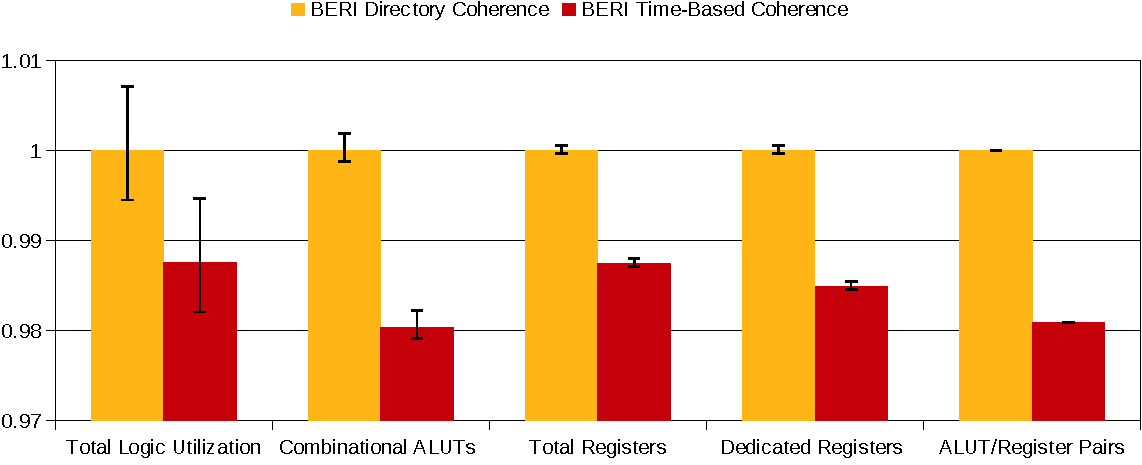
\includegraphics[trim={0 0cm 0 0cm},clip,width=\textwidth,height=\textheight,keepaspectratio]{quartus_graph}}
			\caption[Normalised Quartus overheads]{Normalised Quartus overheads (\textit{Note: The total logic utilization is derived from a complete FPGA design synthesis. Registers and ALUTs show CPU overheads})} 
			\label{quartus_graph}
		\end{figure}	
		

\begin{comment}
		\begin{table}[!h]	
		\centering
		\resizebox{\textwidth}{!}{\begin{tabular}{|l||c|c||c|}
			\hline
			\multicolumn{4}{|c|}{Quartus II 64-Bit -- Version 13.1.0} \\
			\multicolumn{4}{|c|}{Family Stratix IV} \\
			\multicolumn{4}{|c|}{Device -- EP4SGX230KF40C2} \\
			\hline
			Statistic & Directory & Time-Based & FPGA Capacity \\
			\hline 
			\hline
			Total Logic Utilization & 105,720 (58\%) & 104,404 (57.2\%) &  182,400 \\
			Combinational ALUTs & 71,723 (39.3\%) & 70,312 (38.5\%) & 182,400 \\
			Total Registers & 65,456 & 64,637 & 14,625,792 \\
			Dedicated Registers & 65,059 & 64,076 & 14,625,792 \\
			Total BRAM Bits & 3,833,174 & 3,796,310 & 14,625,792 \\
			ALUT/Register Pairs & 101,134 & 99,205 & --- \\
			%\hline
			%Total combinational functions & 71,329 & 69,934 & ? \\
			%-- 7 input functions & 1,206 & 1,209 & ? \\
			%-- 6 input functions & 20,908 & 20,417 & ? \\
			%-- 5 input functions & 13,225 & 13,955 & ? \\
			%-- 4 input functions & 12,113 & 11,996 & ? \\
			%-- <=3 input functions & 23,877 & 22,357 & ? \\
			Clustering Difficulty & Low & Low & NA \\
			\hline
		\end{tabular}}
		\caption{Dual-core BERI FPGA Resource Overhead Comparison (Mean)}
		\label{fpga_other_overheads}
		\end{table}
\end{comment}

\clearpage
\section{Application of Time-Based Coherence }
	\label{section_application_timebased}
	So far I have highlighted the properties of time-based coherence. A major advantage of the time-based model is its implementation simplicity, design modularity and lower hardware overheads.
	
	\paragraph{Simplicity}
		This model can be implemented in designs where a dedicated coherence network is undesirable. Any drawbacks of cache self-invalidation may outweigh the design complexity of a message based coherence protocol. 
			
	\paragraph{Usability}
		This model is supported by the widely used FreeBSD operating system. The protocol could be adapted for other operating systems supporting weak consistency, such as Debian GNU/Linux \cite{Merrill03}.
	
	\paragraph{Scalability}
		The multiprocessor evaluation of time-based coherence has been limited by the FPGA size. However, the obtained results permit some speculation. The minimum requirement for the time-based protocol would be some form of consistency in the shared memory/network. Coherence is implemented directly in the private caches, thus, no additional network or communication is required and cores can be plugged directly into the shared fabric. 
		Optimisations such as detection of polling operations and more sophisticated versions may eliminate timestamps all together, leading to a SYNC-only based design.
		
		This coherence scheme could be implemented on small clusters of general purpose cores, sharing a common memory. For instance, tiled chip-multiprocessors.
		Some relevant examples are: (1) MasPar MP-1 \cite{maspar90}, a good example of early work on building multiprocessors. This design consists of multiple processor boards communicating through a network. Each board contains a cluster of cores. (2) The Intel 48-core SCC \cite{Mattson10} processor is based on a tiled design, where each tile holds a pair of processor cores. The two cores can communicate using time-based coherence, while other protocols can be applied to the rest of the network. (3) The Godson-3 processor \cite{godson3} consists of interconnected nodes. Each node contains 4 cores, sharing a bank of L2 caches. Time-based coherence can be used within a node.

		The coherence protocol can be applied to systems with persistent memory, where time-based self-invalidation would work in tandem with requirements to selectively flush data to persistent storage. HP's `The Machine' project \cite{hp_the_machine} is one such example. Coherence support for this system is currently absent and a simple time-based approach could be beneficial.



















%CHAPTER **************************************************************************
%CHAPTER **************************************************************************
%CHAPTER **************************************************************************
%CHAPTER **************************************************************************
%CHAPTER **************************************************************************

\chapter{Memory Consistency Verification}
\label{chapter_validation}

		Litmus tests are an emerging way for architects to evaluate the memory consistency model of a given processor architecture; demonstrated by Alglave et al. \cite{Alglave11}. These tests typically consist of very short parallel memory operations spread over multiple cores, designed to identify subtle variations in memory consistency. Tests evaluate all permutations for a given set of memory instructions. 
		%The AXE test suite \cite{AXE_checker,bluecheck} is a collection of Litmus style tests executed recursively with injection of additional memory instructions. 
		
		The BERI multiprocessor designs are analysed using the AXE memory checking tool in a triple-core set-up, increasing the interleaving of memory operations. 
		This set-up improves the robustness of model evaluation, while also permitting reasonably short simulation times. The AXE observations are further backed by CHERI Litmus tests, designed by Matthew Naylor \cite{CHERI_litmus}. 
		%The performance of the time-based and directory-based designs is evaluated in simulation using Litmus tests (Section \ref{litmus_perfromance}).
		
		In this chapter I will discuss the memory consistency behaviour of time-based coherence, followed by an analysis of the directory-based model, and conclude with a simple performance evaluation using the aforementioned tools.


\section{Verifying BERI Time-Based Coherence}
		The unique behaviour of time-based coherence differentiates it from other relaxed memory models. While systems such as PowerPC state a number of memory consistency properties, not all of these may be visible in hardware. This is due to variations in cache design, memory latency, reordering of instructions, cache optimisations, and many other factors.
		
		In this section I discuss a small selection of interesting observable, non-observable, and forbidden time-based consistency scenarios. The examples use the memory format previously described in Section \ref{mem_format}.

\clearpage
		\subsection{Observable Relaxed Behaviour}
		In this section we look at several relaxed memory consistency scenarios observed on BERI time-based coherence but not observed on the PowerPC memory model. 
		There are many more observable examples but only a few are shown.
		The PowerPC model is illustrated in work by Sarkar et al. and Maranget et al. \cite{Sarkar11,Maranget12}.
		Note that the notion of threads and cores is equivalent for all examples shown in this section.
		%Other scenarios where the PowerPC model and time-based model exhibit similar behaviour are also shown.
		
%Example
%\newpage						
\paragraph{Test (MP+sync+dep)}
		%This example is observable on the time-based model but not on PowerPC \cite{Sarkar11,Maranget12}. 
		Time-based coherence allows stale data to reside in the cache, thus loads to stale memory are allowed. The example shown in Figure \ref{mp_sync_dep_diagram} demonstrates the stated behaviour.
		
		Steps \textbf{(a:)} and \textbf{(b:)} on Thread 0 are both store operations, the former is propagated using the SYNC instruction. The stores update values of \textbf{(x)} and \textbf{(y)} respectively. Thread 1 at step \textbf{(c:)} is dependent on the store at \textbf{(b:)}. The final operation at \textbf{(d:)} is the load of \textbf{(x)}, and loading the initial value is acceptable.
		
		If we assume a sequential memory behaviour with no stale data caching, then the load of \textbf{(x)} at \textbf{(d:)} would always produce an updated value. For our time-based system, the load at \textbf{(d:)} can produce either the original or the updated value of \textbf{(x)}. 
		A valid tag-time-stamp would allow the initial value to reside in the local cache.
		%since the original value can be held in the private cache with a valid tag-time-stamp.

\begin{figure}[!h]
\begin{tcolorbox}[
colback=green!1!white,
colframe=green!75!black]
\begin{center}
\begin{BVerbatim}
*  Memory Operations  *
0: M[0] := 1
0: sync
0: M[1] := 1
1: M[1] == 1 (blocking)
1: M[0] == 0
\end{BVerbatim}
\end{center}		
%\caption{MP+sync+dep.axe}
%\label{mp_sync_dep_instructions}

\centering
\begin{tabular}{|c|c|c|}
\hline
po: program order & dep: dependency (blocking) & rf: read from \\
\hline
\end{tabular}
\vspace{-9mm}

\begin{displaymath}
	\xymatrix{
		Thread \ 0 & \ \ \ \ \ \  & Thread \ 1 \\
		a: W[x] = 1 \ar[d]_{po} & & c: R[y] = 1 \ar[dd]^{dep} \\
		sync \ar[d]_{po} & \ \ \ \ar@2{~>}[dr]^{rf} & \\
		b: W[y] = 1 \ar@/^/@{->}[uurr]^{rf} & & d: R[x] = 0
	}
\end{displaymath}
\end{tcolorbox}
\caption{Test (MP+sync+dep)}
\label{mp_sync_dep_diagram}
\end{figure}

\clearpage
		Step \textbf{(c:)} may produce an updated value, since its data copy could have expired in the private cache. Systems relying on coherence messages may not exhibit this behaviour, since eager coherence messaging will evict stale memory locations. However, systems using lazy coherence messaging along with message reordering might produce a similar outcome.

%Example
%\newpage
\paragraph{Test (WRC+sync+dep)}
		%This example is observable on the time-based model but not on PowerPC. 
		
		Figure \ref{wrc_sync_dep_diagram} shows a triple thread Litmus test evaluating coherence locality, since local core clusters may exhibit stronger consistency than the whole system. 
		
		Thread 0 performs a store to \textbf{(x)} at \textbf{(a:)}, which is observed by Thread 1 at \textbf{(b:)}. Thread 1 proceeds to execute a SYNC instruction followed by a store to \textbf{(y)} at \textbf{(c:)}. The conditions between steps \textbf{(c:)}, \textbf{(d:)} and \textbf{(e:)} are identical to the previous example (MP+sync+dep). As we have already observed, when the load of \textbf{(y)} at \textbf{(d:)} yields the latest value, load of \textbf{(x)} at \textbf{(e:)} may still produce stale data. This test shows that Thread 1 observes the memory operation of Thread 0, but Thread 2 does not, despite a flat core layout. This test can be extended to more than three threads while demonstrating the same outcome.
		
\begin{figure}[!h]
\begin{tcolorbox}[
colback=green!1!white,
colframe=green!75!black]
\begin{center}
\begin{BVerbatim}
*  Memory Operations  *
0: M[0] := 1
1: M[0] == 1
1: sync
1: M[1] := 1
2: M[1] == 1 (blocking)
2: M[0] == 0
\end{BVerbatim}
\end{center}
%\caption{WRC+sync+dep.axe}
%\label{wrc_sync_dep_instructions}

\vspace{1mm}

\begin{displaymath}
	\xymatrix{
		Thread \ 0 & \ \ \ \ \ \  & Thread \ 1  & \ \ \ \ \ \  & Thread \ 2\\
		a: W[x] = 1 \ar@/^/@{->}[rr]^{po} & & b: R[x] = 1 \ar[d]_{po} & & d: R[y] = 1 \ar[dd]^{dep} \\
		& & sync \ar[d]_{po} & \ \ \ \ar@2{~>}[dr]^{rf} & \\
		& & c: W[y] = 1 \ar@/^/@{->}[uurr]^{rf} & & e: R[x] = 0
	}
\end{displaymath}
\end{tcolorbox}
\caption{Test (WRC+sync+dep)}
\label{wrc_sync_dep_diagram}
\end{figure}


%Example
\clearpage	
\paragraph{Test (W+RWC+sync+dep+sync)}
		%This example is observable on the time-based model but not on PowerPC.
		Figure \ref{w_rwc_sync_dep_diagram}, shows an example where two threads can observe each others memory operations, but without explicit dependencies other threads may not. 
		
		Thread 0 performs two store operations at \textbf{(a:)} and \textbf{(b:)}, the former enforced through a SYNC. Thread 1 performs two loads at \textbf{(c:)} and \textbf{(d:)}, enforced through a dependency. The interaction between Threads 0 and 1 is allowed and expected under BERI time-based coherence. Thread 2 performs a store at \textbf{(e:)}, enforced by a sync and followed by a load of \textbf{(x)} at \textbf{(f:)}.
		
		Thread 2 is not explicitly dependant on any operations performed by either Thread 0 or 1, and it is free to load the stale value of \textbf{(x)} from its private cache. Additionally, Threads 0 and 1 do not explicitly depend on Thread 2.
		
		This example highlights the behaviour of clustered processor architectures, where closely located cores may display different consistency behaviour to those far apart.
		The example previously shown in Figure \ref{wrc_sync_dep_diagram} [Test (WRC+sync+dep)] demonstrates a similar core clustering behaviour using a different set of dependencies. 

\begin{figure}[!h]
\begin{tcolorbox}[
colback=green!1!white,
colframe=green!75!black]
\begin{center}
\begin{BVerbatim}
*  Memory Operations  *
0: M[0] := 1
0: sync
0: M[1] := 1
1: M[1] == 1 (blocking)
1: M[2] == 0
2: M[2] := 1
2: sync
2: M[0] == 0
\end{BVerbatim}
\end{center}
%\caption{W+RWC+sync+dep+sync.axe}
%\label{w_rwc_sync_dep_instructions}

\vspace{1mm}

\begin{displaymath}
	\xymatrix{
		Thread \ 0 & \ \ \ \ \ \  & Thread \ 1  & \ \ \ \ \ \  & Thread \ 2\\
		a: W[x] = 1 \ar[d]_{po} & & c: R[y] = 1 \ar[dd]^{dep} & & e: W[z] = 1 \ar[d]^{po} \\
		sync \ar[d]_{po} & & & \ \ \ \ar@2{~>}[dr]^{rf} & sync \ar[d]^{po} \\
		b: W[y] = 1 \ar@/^/@{->}[uurr]^{rf} & & d: R[z] = 0 & & f: R[x] = 0
	}
\end{displaymath}
\end{tcolorbox}
\caption{Test (W+RWC+sync+dep+sync)}
\label{w_rwc_sync_dep_diagram}
\end{figure}

\clearpage
	\subsection{Non-Observable Relaxed Behaviour}
		Relaxed memory consistency without dependencies allows a range of memory behaviours. This example is one of several behaviours allowed by RMO{\large$^\star$} but not displayed by BERI time-based coherence.
%Example
\paragraph{Test (LB+sync+dep)}
		Figure \ref{lb_sync_dep_diagram} shows a cyclic dependency between all memory operations. While blocking instructions are largely implementation dependent, SYNC instructions must provide stronger ordering guarantees. SYNC must guarantee that all preceding memory operations (specifically stores) have been completed. Note that SYNC instructions only apply to the executing thread, they are not expected to propagate memory operations from other threads. 
		
		In this example, \textbf{(b:)} occurs after a SYNC operation, thus it cannot complete before \textbf{(a:)} is observed. Step \textbf{(c:)} is a blocking operation depending on the outcome of \textbf{(b:)}, so \textbf{(d:)} cannot happen before \textbf{(c:)}. Step \textbf{(a:)} expects an update from \textbf{(d:)} and cannot succeed without it.
		
		While RMO{\large$^\star$} allows this behaviour, the BERI memory subsystem cannot produce this ordering outcome.
		It is difficult to suggest a hardware design that would exhibit this behaviour; removing the dependency at \textbf{(c:)} would make it possible. 
		

\begin{figure}[!h]
\begin{tcolorbox}[
colback=orange!1!white,
colframe=orange!75!white]
\begin{center}
\begin{BVerbatim}
*  Memory Operations  *
0: M[0] == 1
0: sync
0: M[1] := 1
1: M[1] == 1 (blocking)
1: M[0] := 1
\end{BVerbatim}
\end{center}

\vspace{1mm}

\begin{displaymath}
	\xymatrix{
		Thread \ 0 & \ \ \ \ \ \  & Thread \ 1 \\
		a: R[x] = 1 \ar[d]_{po} & & c: R[y] = 1 \ar[dd]^{dep} \\
		sync \ar[d]_{po} & & \\
		b: W[y] = 1 \ar@/^/@{->}[uurr] & & d: W[x] = 1 \ar@/_/@{->}[uull]^{rf}
	}
\end{displaymath}
\end{tcolorbox}
\caption{Test (LB+sync+dep)}
\label{lb_sync_dep_diagram}
\end{figure}

\clearpage
		\subsection{Forbidden Behaviour} 
		So far I have shown evidence that the time-based memory model is relaxed and exhibits more relaxed behaviour than some commercial hardware \cite{Maranget12}. The next example demonstrates that this coherence model can still provide strong programmer assurances.

%\newpage
\paragraph{Test (MP+syncs)}
		Figure \ref{mp_sync_diagram} shows that adequate use of SYNC instructions is sufficient for correct software behaviour. In this example, individual threads perform operations enforced through SYNCs. 
		
		Thread 0 updates values of \textbf{(x)} and \textbf{(y)} at \textbf{(a:)} and \textbf{(b:)}, and Thread 1 loads \textbf{(x)} and \textbf{(y)} at \textbf{(c:)} and \textbf{(d:)}. If Thread 1 observes the updated value of \textbf{(y)} then it will also observe the updated value of \textbf{(x)}, the SYNC instruction will guarantee stale data eviction from private caches (\textit{figure shows memory observations that would result in test failure}). 
		Software written for relaxed consistency systems heavily relies on the behaviour demonstrated in this test, FreeBSD uses this communication style. 
		Each SYNC instruction causes an L1 cache flush, and BERI L1 caches are write-through, so the Thread 0 SYNC is actually unnecessary and can be removed.
		%so overusing it is not recommended.
		
\begin{figure}[!h]
\begin{tcolorbox}[
colback=red!1!white,
colframe=red!85!black]
\begin{center}
\begin{BVerbatim}
*  Memory Operations  *
     0: M[0] := 1
     0: sync
     0: M[1] := 1
     1: M[1] == 1
     1: sync
     1: M[0] == 0
\end{BVerbatim}
\end{center}
%\caption{MP+syncs.axe}
%\label{mp_sync_instructions}

\vspace{2mm}

\begin{displaymath}
	\xymatrix{
		Thread \ 0 & \ \ \ \ \ \  & Thread \ 1 \\
		a: W[x] = 1 \ar[d]_{po} & & c: R[y] = 1 \ar[d]^{po} \\
		sync \ar[d]_{po} & \ \ \ \ar@2{~>}[dr]^{rf} & sync \ar[d]^{po} \\
		b: W[y] = 1 \ar@/^/@{->}[uurr]^{rf} & & d: R[x] = 0
	}
\end{displaymath}
\end{tcolorbox}
\caption{Test (MP+syncs)}
\label{mp_sync_diagram}
\end{figure}


\clearpage
% % % % % % % % % % % % % % % % % % % % % % % % % % % % % % % % % % % % % % % % % %
	\subsection{CHERI Litmus Tests}
		\label{cheri_litmus_tests}
		Litmus tests are a way of testing whether specific concurrent behaviours are actually observable in hardware. Unlike the AXE evaluation, which tests the memory subsystem hardware in isolation, these are assembley-language (software) tests that run on the CPU. CHERI Litmus \cite{CHERI_litmus} is a tool that takes a Litmus test and turns it into a software program that repeatedly (1) randomises the variable locations, (2) synchronises the cores, (3) inserts random delays, (4) executes the Litmus test, (5) checks the Litmus test condition, and (6) records the results.
		
		Message passing (MP) with SYNCs has already been presented in Figure \ref{mp_sync_dep_diagram} [Test (MP+sync+dep)], a similar scenario is demonstrated in this section using CHERI Litmus. We observe different memory consistency behaviour depending on the use of SYNCs. The default Litmus MP test does not use SYNC instructions. Lack of SYNCs and a long self-invalidation time-out will ensure that stores from other threads will not be observed. 
		
		Three tests are evaluated: MP1-default, MP1-SYNC, and MP2. Two versions of the MP1 test were created in order to observe all outcomes. The barrier implementation required by the test also plays a major role. The MP2 test uses a SYNC instruction between the two load operations of thread 1, this test mimics the example shown in Figure \ref{mp_sync_diagram} [Test (MP+syncs)]. Time-based coherence guarantees that the specified outcomes will not be observed.

\begin{figure}[t]
\begin{tcolorbox}[
colback=blue!1!white,
colframe=blue!65!black]
\begin{center}
% {0:r2=x; 0:r4=y; 1:r2=x; 1:r4=y;}
\begin{BVerbatim}
        Initial Conditions       
(r2 = address x; r4 = address y;)
Test Condition (1:r3=1 /\ 1:r1=0)

         P0              P1 
1:  li r1,1      |  lb  r3,0(r4) 
2:  sb r1,0(r2)  |  lb  r1,0(r2) 
3:  sb r1,0(r4)  |
4:  sync*        |
\end{BVerbatim} 
\end{center}
\end{tcolorbox}
\caption[Message passing 1, default and modified tests]{Message passing 1, default and modified tests (*optional)}
\label{mp_1_litmus}
\end{figure}

\begin{figure}[!h]
\begin{tcolorbox}[
colback=blue!1!white,
colframe=blue!65!black]
\begin{center}
%{0:r2=x; 0:r4=y; 1:r2=x; 1:r4=y;}
\begin{BVerbatim}
        Initial Conditions       
(r2 = address x; r4 = address y;)
Test Condition (1:r3=1 /\ 1:r1=0)

         P0              P1 
1:  li r1,1      |  lb  r3,0(r4) 
2:  sb r1,0(r2)  |  sync 
3:  sync         |  lb  r1,0(r2) 
4:  sb r1,0(r4)  | 
\end{BVerbatim}
\end{center}
\end{tcolorbox}
\caption{Message passing 2, default test}
\label{mp_2_litmus}
\end{figure}

		Figure \ref{mp_1_litmus} shows the code sequence used in the MP1 test. The default test is executed without the SYNC instruction (line 4). In the modified test, the SYNC instruction in added into the sequence. Figure \ref{mp_2_litmus} shows the MP2 test. The two SYNC instructions (P0: line 3 and P1: line 2), ensure that this condition is never observed on time-based coherence.

		The barrier loop implemented in CHERI Litmus is shown in Figure \ref{barrier_litmus}. The SYNC instruction (line 6) is not present in the default case. 
		This instruction has been added to observe the desired memory states and to improve the overall execution time on the time-based model. 
		The barrier contains two loops: one is dependant on LL/SC instructions, and the second relies on shared memory updates. 
		
		This code uses a polling technique to wait for memory updates. Lines will be locally cached until the timer expires, and depending on the time-out, this loop could take a long time to execute. The SYNC instruction ensures that fresh data copies are fetched more frequently.
		
		If SYNC instructions are omitted, the time-based model with a simple polling detection mechanism can be used, it speeds-up overall performance while maintaining the correct consistency model.
		
\begin{figure}[!h]
\begin{tcolorbox}[
colback=violet!1!white,
colframe=violet!75!black]
\begin{center}
\begin{BVerbatim}
1:  lld    $8, 0(%0)  < :: :: :: ::
2:  daddu  $8, $8, %1            ::
3:  scd    $8, 0(%0)             ::
4:  beqz   $8, 1b     {Branch to 1}
5:  nop
6:  sync*             < :: :: :: ::
7:  ld     $8, 0(%0)             ::
8:  bne    $8, %2, 6b {Branch to 6}
9:  nop
10: sync
\end{BVerbatim} 
\end{center}
\end{tcolorbox}
\caption{Barrier implementation}
\label{barrier_litmus}
\end{figure}
		
\begin{table}[!ht]
\centering
\resizebox{\textwidth}{!}{\begin{tabular}{c|c|c|l|c|c|c|c|}
\cline{2-8} 
& Modified & Polling & \multicolumn{1}{|c|}{Coherence} & \multicolumn{4}{ c| }{Observed Outcomes} \\ 
\cline{5-8}
& Barrier & Detection & \multicolumn{1}{|c|}{Model} & r3=1 & r3=0 & r3=0 & r3=1 \\
& & & & r1=1 & r1=1 & r1=0 & r1=0 \\
\hhline{-=======}
\multicolumn{1}{|c }{\multirow{4}{*}{\parbox{1.6cm}{\centering MP1 Default}}} &
\multicolumn{1}{|c|}{} & \multicolumn{1}{|c|}{} & Time-Based & 0 & 0 & \textbf{\textcolor{Bittersweet}{1000}} & 0 \\
\multicolumn{1}{|c }{} &
\multicolumn{1}{|c|}{$\bullet$} & \multicolumn{1}{|c|}{} & Time-Based & 81 & 18 & 895 & \textbf{\textcolor{Fuchsia}{6}} \\
\multicolumn{1}{|c }{} &
\multicolumn{1}{|c|}{} & \multicolumn{1}{|c|}{$\ast$} & Time-Based & 321 & 89 & 582 & \textbf{\textcolor{Fuchsia}{8}} \\
\multicolumn{1}{|c }{} &
%\multicolumn{1}{|c|}{$\bullet$} & Time-Based (poll-detect) & 152 & 34 & 801 & \textbf{13} \\
%\multicolumn{1}{|c }{} &
\multicolumn{1}{|c|}{} & \multicolumn{1}{|c|}{} & Directory & 517 & 107 & 376 & 0 \\
\multicolumn{1}{|c }{} &
\multicolumn{1}{|c|}{$\bullet$} & \multicolumn{1}{|c|}{} & Directory & 620 & 101 & 279 & 0 \\
\hline
\multicolumn{1}{|c }{\multirow{4}{*}{\parbox{1.6cm}{\centering MP1 SYNC}}} &
\multicolumn{1}{|c|}{} & \multicolumn{1}{|c|}{} & Time-Based & 271 & 0 & 729 & 0 \\
\multicolumn{1}{|c }{} &
\multicolumn{1}{|c|}{$\bullet$} & \multicolumn{1}{|c|}{} & Time-Based & 71 & 5 & 913 & \textbf{\textcolor{Fuchsia}{11}} \\
\multicolumn{1}{|c }{} &
\multicolumn{1}{|c|}{} & \multicolumn{1}{|c|}{$\ast$} & Time-Based & 342 & 77 & 576 & \textbf{\textcolor{Fuchsia}{5}} \\
\multicolumn{1}{|c }{} &
%\multicolumn{1}{|c|}{$\bullet$} & Time-Based (poll-detect) & 155 & 40 & 795 & \textbf{10} \\
%\multicolumn{1}{|c }{} &
\multicolumn{1}{|c|}{} & \multicolumn{1}{|c|}{} & Directory & 543 & 72 & 385 & 0 \\
\multicolumn{1}{|c }{} &
\multicolumn{1}{|c|}{$\bullet$} & \multicolumn{1}{|c|}{} & Directory & 623 & 22 & 355 & 0 \\
\hline 
\multicolumn{1}{|c }{\multirow{4}{*}{\parbox{1.6cm}{\centering MP2 Default}}} &
\multicolumn{1}{|c|}{} & \multicolumn{1}{|c|}{} & Time-Based & 49 & 43 & 908 & 0 \\
\multicolumn{1}{|c }{} &
\multicolumn{1}{|c|}{$\bullet$} & \multicolumn{1}{|c|}{} & Time-Based & 95 & 43 & 862 & 0 \\
\multicolumn{1}{|c }{} &
\multicolumn{1}{|c|}{} & \multicolumn{1}{|c|}{$\ast$} & Time-Based & 261 & 297 & 442 & 0 \\
\multicolumn{1}{|c }{} &
%\multicolumn{1}{|c|}{$\bullet$} & Time-Based (poll-detect) & 137 & 117 & 746 & 0 \\
%\multicolumn{1}{|c }{} &
\multicolumn{1}{|c|}{} & \multicolumn{1}{|c|}{} & Directory & 529 & 115 & 356 & 0 \\
\multicolumn{1}{|c }{} &
\multicolumn{1}{|c|}{$\bullet$} & \multicolumn{1}{|c|}{} & Directory & 627 & 124 & 249 & 0 \\
\hline
\end{tabular}}
\caption{Litmus: Message passing, observed outcomes}
\label{litmus_table}
\end{table}	

		The test outcomes for MP1-default, MP1-SYNC and MP2 are documented in Table \ref{litmus_table}. This table shows the outcomes of a 1,000 iterations of the Litmus tests in simulation. A cache line lifetime of 10,000 cache cycles is used to produce the displayed results. It is evident that all combinations of register outcomes are only observed in MP1-default and MP1-SYNC, matching the expected behaviour. 
		
		%The tests are highly timing sensitive and achieving all outcomes required some adjustments, however, no modifications were made to the hardware. 		
		An interesting test outcome is observed when the default MP1 test in executed with the default barrier implementation. The output registers constantly read the initial values, since the time-counter does not expire for the entire duration of this test.
		
		The time-based model with polling detection does not require any additional SYNCs to demonstrate the desired outcome. The barrier loop does not rely on cache line time-outs, as the hardware will detect polling and automatically update the line, improving performance and simplifying the observations.

		The Litmus tests were also executed on the directory version of BERI, the results are presented in the same table. Notably the directory model demonstrates a stronger consistency model and the final output (r3=1, r1=0) is never observed, as expected in TSO behaviour. Majority of time-based coherence results display initial value loads, whereas the directory results show a greater number of fully updated or transitional values.

%\clearpage
	\subsection{AXE Trace Evaluation}
		So far I have discussed the behaviour of time-based coherence using specific memory access patterns. While Litmus testing searches for particular
		small examples of RMO, the AXE tool checks
		arbitrary memory traces for consistency, giving further assurances
		about correctness. AXE is used in a hardware testing
		framework where the memory subsystem can be exercised more thoroughly
		than may be possible via software tests running on the processor. The analysis shows why the time-based coherence model complies with RMO{\large$^\star$} and does not meet the requirements of stronger models. The example traces follow the trace format shown in Section \ref{mem_format}.
		
		When AXE detects a consistency failure, the hardware test framework
		proceeds to reduce the number of instructions, weeding out inconsequential or irrelevant instructions, until the failure is no longer observable. All the minimal examples shown here are a product of this reduction process, as a result, the failing traces display significant time gaps where the
		instructions have been automatically removed.

%\clearpage
		\subsubsection{Sequential Consistency Test}
			The test sequence shown in Trace \ref{sc_test_mem} is an extract of an AXE trace, displaying a violation of the SC model by a software simulation of BERI time-based coherence. 
			
			At time 0, core 0 loads the initial value of variable \textbf{(x)}. In the next cycle, core 1 updates the value of \textbf{(x)}. According to sequential consistency, any core loading the value of \textbf{(x)} in any following cycles must observe the latest store value. After several dead cycles, at time 7, core 1 loads the initial value of \textbf{(y)}. A few cycles later, at time 15, core 0 updates the value of \textbf{(y)}. 
			
			The two memory operations on \textbf{(y)} do not violate any SC properties, instead they are introduced as independent memory instructions between operations on \textbf{(x)}. Finally, at time 21, 20 cycles after the first update of \textbf{(x)}, core 0 loads the initial value, violating SC. The reason for this behaviour is that caching of stale values is permitted by BERI time-based coherence.
			
			\captionsetup[table]{name=Trace}
			\begin{table}[!h]
			\begin{center}
			\fontfamily{pcr}\selectfont
			\begin{tabular}{|r|l|l|}
				\hline
				\textbf{Time} & \textbf{Testing SC model} & \multicolumn{1}{c|}{\textbf{Comments}} \\
				\hline 
				Init & \multicolumn{1}{c|}{x==0, y==0} & \\
				& & \\
				0 & $\gg$ 0: x == 0 & core[0].op(LW,addr[0]) \\	
				1 & $\gg$ 1: x := 1 & core[1].op(SW,addr[0]) \\
				7 & $\gg$ 1: y == 0 & core[1].op(LW,addr[1]) \\
				15 & $\gg$ 0: y := 1 & core[0].op(SW,addr[1]) \\
				21 & $\gg$ \textbf{\textcolor{Red}{0: x == 0}} & core[0].op(LW,addr[0]) \\
				& $\gg$ \textbf{\textcolor{Red}{Failed!}} & \\
				\hline
			\end{tabular}
			\caption{AXE: SC evaluation}
			\label{sc_test_mem}
			\end{center} 
			\end{table}
			\captionsetup[table]{name=Table}

			\begin{comment}
			% Raw
			setAddrMap(< 8,  7,  2,  1>)
			chooseVars(<V 0x6 0xf 0xe 0x0  >)
			2061: core[0].op(LW,'h3)
			2062: core[2].op(SW,'h3)
			2068: core[2].op(LW,'h0)
			2076: core[0].op(SW,'h0)
			2082: core[0].op(LW,'h3)
			0: v0 == 0
			2: v0 := 10
			2: v6 == 0
			0: v6 := 8
			0: v0 == 0
			Failed!
			
			\end{comment}

			SC is a very strong model, rarely enforced by hardware, as it imposes strict ordering on memory operations, implementing this behaviour may be difficult or impractical. Additionally, a strong model does not result in a better cache performance, since every shared data store will likely block all other memory operations, resulting in pipeline stalls.

		\subsubsection{Total Store Order Consistency Test}
			Similar to the SC evaluation, an example of the TSO consistency violation is shown in Trace \ref{tso_test_mem}.
			
			At time 0, core 0 loads the initial value of variable \textbf{(x)}. At time 4, core 1 updates the value of \textbf{(x)}, after a few dead cycles, the same core updates the value of \textbf{(y)} (time 12). At this point both memory locations \textbf{(x)} and \textbf{(y)} have been updated. Loading of stale values from either location is not permitted by SC, however, TSO permits stale loads as long as the ordering of stores has not been violated. 
			
			At time 15, core 0 observes the updated value of \textbf{(y)}, indicating that any stale copies of the variable have been evicted from its privet cache. However, 33 cycles later, at time 48, the same core loads the initial value of \textbf{(x)}, violating TSO. The trace would pass TSO under these circumstances:
			
			\begin{enumerate}
				\item If the final load of \textbf{(x)} preceded the updated load of \textbf{(y)}, the behaviour would satisfy TSO.
				\item If the memory instructions were to be executed in the same sequence, only an updated load of \textbf{(x)} would satisfy TSO.
			\end{enumerate}
			 
			\captionsetup[table]{name=Trace}
			\begin{table}[!h]
			\begin{center}
			\fontfamily{pcr}\selectfont
			\begin{tabular}{|r|l|l|}
				\hline
				\textbf{Time} & \textbf{Testing TSO model} & \multicolumn{1}{c|}{\textbf{Comments}} \\
				\hline 
				Init & \multicolumn{1}{c|}{x==0, y==0} & \\
				& & \\
				0 & $\gg$ 0: x == 0 & core[0].op(LW,addr[0]) \\
				4 & $\gg$ 1: x := 1 & core[1].op(SW,addr[0]) \\
				12 & $\gg$ 1: y := 1 & core[1].op(SW,addr[1]) \\
				15 & $\gg$ \textbf{\textcolor{ForestGreen}{0: y == 1}} & core[0].op(LW,addr[1]) \\
				48 & $\gg$ \textbf{\textcolor{Red}{0: x == 0}} & core[0].op(LW,addr[0]) \\
				& $\gg$ \textbf{\textcolor{Red}{Failed!}} & \\
				\hline
			\end{tabular}
			\caption{AXE: TSO evaluation}
			\label{tso_test_mem}
			\end{center} 
			\end{table}
			\captionsetup[table]{name=Table}
			
			\begin{comment}
			%Raw
			setAddrMap(<10,  8,  6,  0>)
			chooseVars(<V 0x8 0xd 0xa 0xf  >)
			2062: core[0].op(LW,'h0)
			2066: core[2].op(SW,'h0)
			2074: core[2].op(SW,'h2)
			2077: core[0].op(LW,'h2)
			2110: core[0].op(LW,'h0)
			0: v8 == 0
			2: v8 := 10
			2: v10 := 18
			0: v10 == 18
			0: v8 == 0
			Failed!
			\end{comment}

		The TSO model is widely used in multiprocessor architectures. One such example is x86, its memory model has extensive coherence support which allows relatively fast distribution of coherence messages necessary for TSO consistency.

		\subsubsection{Partial Store Order Consistency Test}
			The PSO memory model is designed to account for write buffers. The buffers allow batching of writes to consecutive memory locations, thus reducing traffic to the private caches. This behaviour is also beneficial for write-through caches, since it minimises the number of updates to shared memory. Loading values from write buffers is permitted and useful when software repeatedly updates and reloads data. PSO consistency allows reordering of stores to independent memory locations. BERI does not use write buffers in either of the architectures and the time-based version fails this test due to caching of stale data. Example shown in Trace \ref{pso_test_mem} demonstrates this behaviour. Unlike the SC and TSO scenarios, here we observe memory interactions between three cores.
			
			At time 0, core 2 loads the initial value of variable \textbf{(x)}. After many dead cycles, at time 43, core 1 loads the initial value of \textbf{(y)}. This operation does not have any significance in the final outcome. At time 45, core 0 updates the value of \textbf{(x)}. 2 cycles after the store operation, core 1 observes the updated value of \textbf{(x)}. This is an important result, indicating that the update has been propagated to shared memory (the two operations on variable \textbf{(z)} are not significant). 41 cycles after core 1 observed the update value of \textbf{(x)}, core 2 (time 88) loads the initial value, violating PSO. Identifying a failure of PSO requires more testing cycles than either SC or TSO as its exhibits a more relaxed behaviour.

			\captionsetup[table]{name=Trace}
			\begin{table}[!h]	
			\begin{center}
			\fontfamily{pcr}\selectfont
			\begin{tabular}{|r|l|l|}
				\hline
				\textbf{Time} & \textbf{Testing PSO model} & \multicolumn{1}{c|}{\textbf{Comments}} \\
				\hline 
				Init & \multicolumn{1}{c|}{x==0, y==0} & \\
				& & \\
				0 & $\gg$ 2: x == 0 & core[2].op(LW,addr[0]) \\
				43 & $\gg$ 1: y == 0 & core[1].op(LW,addr[1]) \\
				45 & $\gg$ 0: x := 1 & core[0].op(SW,addr[0]) \\
				47 & $\gg$ 1: x == 1 & core[1].op(LW,addr[0]) \\
				57 & $\gg$ 1: z := 1 & core[1].op(SW,addr[2]) \\
				72 & $\gg$ \textbf{\textcolor{BurntOrange}{2: z == 1}} & core[2].op(LW,addr[2]) \\
				88 & $\gg$ \textbf{\textcolor{Red}{2: x == 0}} & core[2].op(LW,addr[0]) \\
				& $\gg$ \textbf{\textcolor{Red}{Failed!}} & \\
				\hline
			\end{tabular}
			\caption{AXE: PSO evaluation}
			\label{pso_test_mem}
			\end{center} 
			\end{table}
			\captionsetup[table]{name=Table}

						\begin{comment}
						setAddrMap(< 5,  3,  2,  0>)
						chooseVars(<V 0xa 0x1 0x3 0xf  >)
						%2086: core[1].op(LW,'h1)
						2095: core[2].op(LW,'h3)
						2138: core[1].op(LW,'h0)
						2140: core[0].op(SW,'h3)
						2142: core[1].op(LW,'h3)
						2152: core[1].op(SW,'h2)
						2167: core[2].op(LW,'h2)
						2183: core[2].op(LW,'h3)
						%1: v1 == 0
						2: v15 == 0 %x
						1: v10 == 0 %y
						0: v15 := 8 %x
						1: v15 == 8 %x
						1: v3 := 9 %z
						2: v3 == 9 %z
						2: v15 == 0 %x
						Failed!
						\end{comment}
			
			Desired behaviour could be achieved by inserting a SYNC instruction in the core 2 memory sequence just prior to the final load of \textbf{(x)}. It would cause an eviction of stale data and result in an updated load. Synchronisation instructions are the only way of guaranteeing updated shared memory loads.
			
	\subsection{Regression Testing}
		Extensive AXE verification has confirmed that BERI time-based coherence complies
		with the \textbf{RMO{\large$^\star$}} consistency model (\textit{Note: RMO{\large$^\star$} is a subset of the AXE RMO memory model}). The checker tool has analysed 1,000,000 memory instruction permutations on the coherence model in simulation. Table \ref{time_based_regression} shows memory executions with different parameters. The instruction depth indicates the number of instructions checked for correct consistency behaviour. Each instruction depth was tested with a varying set of instructions, 200 times.
		
		Axe supports checking atomicity of successful LL/SC pairs, the memory subsystem can be stimulated with LL/SC operations (+LLSC) in addition to normal loads and stores. Each model parameter can affect system behaviour. The presence of an LL/SC instruction could affect the time between other memory operations. If a SYNC verification step relies on this timing, an incorrect test success may be declared. In order to avoid such a scenario, the time-based memory consistency scheme was tested with all combinations of test parameters.

		\begin{table}[!b]	
		\begin{center}					
		\begin{tabular}{|l||c|c|c|}
			\hline
			Model Parameters & Instruction Depth & No. of Iterations & Outcome \\ 
			\hline 
			RMO & 5000 & 200 & Pass \\
			RMO +LLSC & 5000 & 200 & Pass \\
			RMO +SYNC & 5000 & 200 & Pass \\
			RMO +LLSC +SYNC & 5000 & 200 & Pass \\
			\hline
		\end{tabular}
		\caption{AXE time-based coherence memory consistency verification}
		\label{time_based_regression}
		\end{center} 
		\end{table}

		AXE aggressively tests the memory subsystem. The tool does not account for the processor pipeline, and the rate of memory operations injected into the caches may be impossible to achieve with a full processor. However, this form of testing allows us to provide very strong grantees on memory behaviour since the worst case is tested. The tool is very efficient at spotting inconsistencies, in most cases a memory model failure is detected with an instruction depth of less than 1,000. Larger instructions depths, exceeding 5000 instructions have also been tested, yielding identical results\footnote{The extended AXE trace evaluation has not been presented here, since it does not provide any new information regarding memory consistency behaviour.}.




\section{Verifying BERI Directory Coherence}
	I have already presented some Litmus results for the BERI directory-based coherence model in Section \ref{cheri_litmus_tests}. In this section I describe the AXE trace evaluation and regression testing of this coherence implementation.

	\subsection{AXE Trace Evaluation}
		The BERI directory-based coherence model enforces TSO consistency. This memory model was selected partly due to related research in the field, Elver and Nagarajan \cite{Elver14}, and partly due to the inherent properties of coherence messaging. The coherence network allows fast and efficient distribution of messages, intentionally degrading the performance of this network in order to achieve a weaker model is unnecessary. 

		The BERI directory passes all but the SC consistency check in our test framework. The example shown in Trace \ref{directory_sc_test_mem} demonstrates an SC compliance failure. This test shows an interaction between three cores. 
		
		At time 0, cores 1 and 2 load initial values of \textbf{(x)} and \textbf{(y)}. In the following cycle, all three cores perform updates. Core 0 updates \textbf{(x)} and both cores 1 and 2 update the value of \textbf{(y)}. The two stores are conflicting, and one will overwrite the other in shared memory. Finally at time 8, cores 0 and 1 observe the initial values of \textbf{(x)} and \textbf{(y)}. This behaviour is not valid in SC but perfectly acceptable in TSO. 
		
		The coherence messages generated by the directory are likely in transit or blocked due to busy private caches. All invalidates are delivered to all sharer cores simultaneously, however, at least one private cache might be in a fetch state, waiting for a memory response or performing another blocking operation. This will result in an invalidation delay. In our caches, all responses must be consumed before proceeding, thus cancelling a fetch midway is not possible.

		\captionsetup[table]{name=Trace}
		\begin{table}[!t]
		\begin{center}
		\fontfamily{pcr}\selectfont
		\begin{tabular}{|r|l|l|}
			\hline
			\textbf{Time} & \textbf{Testing SC model} & \multicolumn{1}{c|}{\textbf{Comments}} \\
			\hline 
			Init & \multicolumn{1}{c|}{x==0, y==0} & \\
			& & \\
			0 & $\gg$ 1: x == 0 & core[1].op(LW,addr[0]) \\
			0 & $\gg$ 2: y == 0 & core[2].op(LW,addr[1]) \\
			1 & $\gg$ 0: x := 1 & core[0].op(SW,addr[0]) \\
			1 & $\gg$ 1: y := 1 & core[1].op(SW,addr[1]) \\
			1 & $\gg$ 2: y := 2 & core[2].op(SW,addr[1]) \\
			8 & $\gg$ \textbf{\textcolor{Red}{0: y == 0}} & core[0].op(LW,addr[1]) \\
			8 & $\gg$ \textbf{\textcolor{Red}{1: x == 0}} & core[1].op(LW,addr[0]) \\
			& $\gg$ \textbf{\textcolor{Red}{Failed!}} & \\
			\hline
		\end{tabular}
		\caption{AXE: SC evaluation}
		\label{directory_sc_test_mem}
		\end{center} 
		\end{table}
		\captionsetup[table]{name=Table}

					\begin{comment}
					setAddrMap(<17, 12, 11,  5>)
					chooseVars(<V 0xb 0xf 0x4 0x2  >)
					%2065: core[0].op(SW,'h3)
					2065: core[1].op(LW,'h0)
					2065: core[2].op(LW,'h2)
					2066: core[0].op(SW,'h0)
					2066: core[1].op(SW,'h2)
					2066: core[2].op(SW,'h2)
					2069: core[0].op(LW,'h2)
					2069: core[1].op(LW,'h0)
					%2069: core[2].op(SW,'h3)
					%0: v2 := 8
					1: v11 == 0 %x
					2: v4 == 0 %y
					0: v11 := 16 %x
					1: v4 := 9 %y
					2: v4 := 10 %y
					0: v4 == 0 %y
					1: v11 == 0 %x
					%2: v2 := 18
					Failed!
					\end{comment}

	
	\subsection{Regression Testing}
		The BERI directory coherence model is verified using AXE, just like the time-based model. The final revision of this coherence scheme has passed all of the tests shown in Table \ref{directory_regression}. Each test simulation ran a total of 1,000,000 iterations before declaring a pass. Using the tool, the memory model has been tuned to comply with TSO for all input test parameters. Any uncertainty in delivery of coherence messages presents a challenge for fine tuning the consistency model, as even a small additional delay may result in failure of TSO and even PSO.
		
		\begin{table}[!h]	
		\begin{center}					
		\begin{tabular}{|l||c|c|c|}
			\hline
			Model Parameters & Instruction Depth & No. of Iterations & Outcome \\ 
			\hline 
			TSO & 5000 & 200 & Pass \\
			TSO +LLSC & 5000 & 200 & Pass \\
			TSO +SYNC & 5000 & 200 & Pass \\
			TSO +LLSC +SYNC & 5000 & 200 & Pass \\		
			\hline
		\end{tabular}
		\caption{AXE directory-based coherence memory consistency verification}
		\label{directory_regression}
		\end{center} 
		\end{table}
		\vspace{-10mm}

%\clearpage
\section{Performance Evaluation Using Litmus}
		\label{litmus_perfromance}
		The execution time of CHERI Litmus tests on time-based and directory models has highlighted some key performance differences. The directory model exhibits strong memory consistency, and memory updates are actively propagated, thus, barrier loops require fewer cycles to complete. The time-based model (without polling detection) takes much longer to run the test, since barrier loops spend a long time waiting for private caches to self-invalidate and update memory locations, as a result the execution time compared to the directory is higher. Appropriate SYNC instructions in the barrier greatly improve performance. The time-based model with polling detection overcomes these penalties, since the cache hardware can detect stale loads and force an update from lower levels of memory.

\begin{figure}[t]
\begin{tcolorbox}[
colback=blue!1!white,
colframe=blue!65!black]
\begin{center}
\begin{BVerbatim}
      P0     |      P1 
1:  li* r1,1 |  li*  r2,1
2:  nop      |  nop 
\end{BVerbatim} 
\end{center}
\end{tcolorbox}
\caption{Litmus NOP test}
\label{nop_litmus}
\end{figure}

		A special NOP instruction test was written to evaluate the performance \footnote{The Litmus tests are evaluated on a dual socket Intel$\textregistered$ Xeon$\textregistered$ CPU E5-2667 v2, with 8 physical and 16 logical cores per socket, operating at 3.30GHz, and a total DRAM capacity of 256GB. The tests are compiled with mips-linux-gnu-gcc Debian 4.4.5-8.}
		(Figure \ref{nop_litmus}). Litmus tests require some register evaluation, hence, two initialisation instructions were added (line 1). Note that these instructions do not interact with memory, and any observed slowdown will be due to the barrier implementation used to synchronise test iterations.
		
		The execution time of the time-based model with a time-out value of 10,000 cycles and no barrier SYNC shows a ($>$32$\times$) slowdown as compared to a directory model. Inserting a SYNC instruction (barrier previously shown in Figure \ref{barrier_litmus}) reduces the slowdown to just over (2$\times$). The relative improvement in the execution time of time-based coherence is ($>$14$\times$). 
		
		At least 5 samples were taken for each test and no more than a 1\% variation in the timing samples was observed for all tests. The cycle accurate simulation produced identical results in each run, so the execution time variation can be attributed to OS behaviour. These results are shown in Table \ref{litmus_nop_performance}. 
		
		The strength of the time-based mechanism lies in correctly crafted code. As we will see in Chapter \ref{coherence_eval}, performance of the optimised coherence mechanism is often equivalent and on occasion better than shown by the directory-based model when running FreeBSD. Additional barrier SYNC instructions have no significant effect on the directory model due to an eager coherence behaviour. There is a small penalty for executing the SYNC instruction but it is negligible compared to other test overheads. 
		%The testing environment used for Litmus testing is described in Table \ref{vaucher_system_info}.
		
		The best performance of the time-based model is achieved when using the cache polling detection mechanism. The private cache is able to determine when an address is polled, thus, a stale location is more frequently updated, and execution time is reduced. Without a barrier SYNC, the polling detection mechanism reduces the total execution time to 85 sec, $\sim$6\% slower than the directory model. The small performance penalty observed is due to self-invalidates and SYNC based cache invalidates. Interestingly, the test version with a barrier SYNC performed worse in this case (98 seconds), as the additional SYNC instruction reduces the cache hit rate. Thus, best performance for the time-based model is achieved when the number of SYNCs and polling operations is well balanced.

		The Litmus testing framework only uses memory instructions and branch instructions, any latency added by the memory subsystem appears more significant when compared to regular application where arithmetic operations are more common. This test framework allows careful analysis of memory behaviour and its effect on overall performance.

		\begin{table} %[!h]
		\begin{center}
		\begin{tabular}{|c|c|c|c|}
		\hline
		Coherence & Modified & Polling & Execution \\
		Model & Barrier & Detection & Time (sec) \\
		\hline
		Time-Based & & & 2575 \\
		Time-Based & $\bullet$ & & 180 \\
		Time-Based & & $\ast$ & 85 \\
		Time-Based & $\bullet$ & $\ast$ & 98 \\
		Directory &  & & 80 \\
		Directory & $\bullet$ & & 80 \\
		\hline
		\end{tabular}
		\caption{Litmus NOP test performance}
		\label{litmus_nop_performance}
		\end{center} 
		\end{table}	


\section{Summary}
	In this chapter I have demonstrated that the BERI time-based coherence model complies with the RMO{\large$^\star$} memory consistency scheme, defined in Chapter \ref{chapter_background}. The directory-based coherence scheme is proven to comply with the TSO memory consistency model. I have also evaluated the basic performance of both coherence models in simulation, using the memory checking tools.




















































































































	
	
	
	
	
\begin{comment}
*** 4 Reg Polling Detector
Observed outcomes:
321: 1:r3=1 1:r1=1 
89: 1:r3=0 1:r1=1 
582: 1:r3=0 1:r1=0 
8: 1:r3=1 1:r1=0 
OBSERVED
real	1m25.138s
user	1m24.969s
sys	0m0.072s

*** 4 Reg Polling Detector + barrier SYNC
Observed outcomes:
152: 1:r3=1 1:r1=1 
34: 1:r3=0 1:r1=1 
801: 1:r3=0 1:r1=0 
13: 1:r3=1 1:r1=0 
OBSERVED
real	1m57.938s
user	1m57.805s
sys	0m0.075s

*** 4 Reg Polling + SYNC
Observed outcomes:
342: 1:r3=1 1:r1=1 
77: 1:r3=0 1:r1=1 
576: 1:r3=0 1:r1=0 
5: 1:r3=1 1:r1=0 
OBSERVED
real	1m29.020s
user	1m28.776s
sys	0m0.084s

*** 4 Reg Polling Detector + SYNC + barrier SYNC
Observed outcomes:
155: 1:r3=1 1:r1=1 
40: 1:r3=0 1:r1=1 
795: 1:r3=0 1:r1=0 
10: 1:r3=1 1:r1=0 
OBSERVED
real	1m42.602s
user	1m42.300s
sys	0m0.084s

MP2 + polling
Observed outcomes:
261: 1:r3=1 1:r1=1 
297: 1:r3=0 1:r1=1 
442: 1:r3=0 1:r1=0 
NOT OBSERVED
real	1m28.618s
user	1m28.435s
sys	0m0.089s

MP2 + polling + barrier sync
Observed outcomes:
137: 1:r3=1 1:r1=1 
117: 1:r3=0 1:r1=1 
746: 1:r3=0 1:r1=0 
NOT OBSERVED
real	1m38.830s
user	1m38.629s
sys	0m0.073s
\end{comment}

	
\begin{comment}
\paragraph{\textbf{AXE Test (LB+dep)}}
		This example (Figure \ref{lb_dep_diagram}) shows a cyclic dependency between all memory operations running on hardware threads. Blocking instructions are largely implementation dependent, BERI time-based coherence permits blocking memory operations to proceed (RMO without dependencies).

		In this example, threads attempt to load values of \textbf{(x)} and \textbf{(y)} at steps \textbf{(a:)} and \textbf{(c:)} respectively. Both load operations are blocking and no new memory operations will be issued until the conditions are satisfied. Steps \textbf{(b:)} and \textbf{(d:)} perform stores to \textbf{(y)} and \textbf{(x)} respectively, these values are required by \textbf{(c:)} and \textbf{(a:)}. Blocking instructions will prevent this sequence form succeeding, unless blocking operations are ignored by the memory subsystem and load/store reordering is permitted. The time-based coherence model does not prevent this scenario, however, the cache structure of BERI does not support out of order execution or reordering of memory instructions.

\begin{figure}[!h]
\begin{tcolorbox}[
colback=orange!1!white,
colframe=orange!75!white]
\begin{center}
\begin{BVerbatim}
*  Memory Operations  *
0: M[0] == 1 (blocking)
0: M[1] := 1
1: M[1] == 1 (blocking)
1: M[0] := 1
\end{BVerbatim}
\end{center}
%\caption{LB+dep.axe}
%\label{lb_dep_instructions}
\vspace{5mm}
%\centering

%\begin{tcolorbox}
\centering
\begin{tabular}{|c|c|c|}
\hline
po: program order & dep: dependency(blocking) & rf: read from \\
\hline
\end{tabular}
\begin{displaymath}
\xymatrix{
	Thread \ 0 & \ \ \ \ \ \  & Thread \ 1 \\
	a: R[x] = 1 \ar[dd]_{dep} & & c: R[y] = 1 \ar[dd]^{dep} \\
	& & \\
	b: W[y] = 1 \ar@/^/@{->}[uurr] & & d: W[x] = 1 \ar@/_/@{->}[uull]^{rf}
}
\end{displaymath}
\caption{AXE Test -- LB+dep}
\label{lb_dep_diagram}
\end{tcolorbox}
\end{figure}
\end{comment}	
	
	
\begin{comment}	
\section{NEW BERI DUAL-CORE WITH ENHANCED CACHES AND COHERENCE}
	The revised version of BERI multi-core has several enhancements. Cache enhancements have been largely credited to Jonathan Woodruff and Alexandre Joannou. The modifications have been largely based on the original version of BERI multi-core. I have added a new Coherence Controller module. This module disassociates the directory from the modular cache. This optimisation allows using the same Bluespec cache modules for all versions of caches: I-Cache, data cache, and L2 (Other levels are possible as well). The Coherence Controller is responsible for keeping a track of sharers and issuing invalidates. The specific workings of the shared cache are masked from the Coherence Controller as this module just observes memory accesses and track data sharing.
	
	\begin{itemize}
	\item All the caches are modular with a number of configurable parameters such as: associativity, capacity, prefetching, out of order behaviour, etc.
	\item The Coherence Controller hold both the directory and the LL/SC resisters.
	\item The data caches perform full lookups for each invalidate, provided the congestion is low. During high congestion phases of operation, the cache simply invalidates the address without a lookup.
	\item The SYNC instruction waits for all outstanding writes to complete before releasing the pipeline. 
	\end{itemize}
\end{comment}


% % % % % % % % % % % % % % % % % % % % % % % % % % % % % % % % % % % % % % % % % % %
\begin{comment}
Tests produce the following histograms:
\begin{table}[!h]	
\begin{center}					
\begin{tabular}{c|l|c|c|c|c|c|}
\cline{2-7} 
& & Approx & \multicolumn{4}{ c| }{Observed Outcomes} \\ 
\cline{4-7}
& \multicolumn{1}{|c|}{Coherence Model} & \multicolumn{1}{c|}{Time} & r3=1 & r3=0 & r3=0 & r3=1 \\
& & \multicolumn{1}{|c|}{(sec)} & r1=1 & r1=1 & r1=0 & r1=0 \\
\hhline{-======}
\multicolumn{1}{|c }{\multirow{4}{*}{\parbox{1.6cm}{\centering MP1 default}}} &
\multicolumn{1}{|l|}{Time-Based} & 2575 & 0 & 0 & \textbf{1000} & 0 \\
\multicolumn{1}{|c }{} &
\multicolumn{1}{|l|}{Time-Based \scriptsize{(B-SYNC)}} & 180 & 81 & 18 & 895 & \textbf{6} \\
\multicolumn{1}{|c }{} &
\multicolumn{1}{|l|}{Directory} & 75 & 517 & 107 & 376 & 0 \\
\multicolumn{1}{|c }{} &
\multicolumn{1}{|l|}{Directory \ \ \ \scriptsize{(B-SYNC)}} & 75 & 620 & 101 & 279 & 0 \\
\hline
\multicolumn{1}{|c }{\multirow{4}{*}{\parbox{1.6cm}{\centering MP1 modified}}} &
\multicolumn{1}{|l|}{Time-Based} & 1380 & 271 & 0 & 729 & 0 \\
\multicolumn{1}{|c }{} &
\multicolumn{1}{|l|}{Time-Based \scriptsize{(B-SYNC)}} & 180 & 71 & 5 & 913 & \textbf{11} \\
\multicolumn{1}{|c }{} &
\multicolumn{1}{|l|}{Directory} & 75 & 543 & 72 & 385 & 0 \\
\multicolumn{1}{|c }{} &
\multicolumn{1}{|l|}{Directory \ \ \ \scriptsize{(B-SYNC)}} & 75 & 623 & 22 & 355 & 0 \\
\hline 
\multicolumn{1}{|c }{\multirow{4}{*}{\parbox{1.6cm}{\centering MP2 default}}} &
\multicolumn{1}{|l|}{Time-Based} & 1465 & 49 & 43 & 908 & 0 \\
\multicolumn{1}{|c }{} &
\multicolumn{1}{|l|}{Time-Based \scriptsize{(B-SYNC)}} & 180 & 95 & 43 & 862 & 0 \\
\multicolumn{1}{|c }{} &
\multicolumn{1}{|l|}{Directory} & 75 & 529 & 115 & 356 & 0 \\
\multicolumn{1}{|c }{} &
\multicolumn{1}{|l|}{Directory \ \ \ \scriptsize{(B-SYNC)}} & 75 & 627 & 124 & 249 & 0 \\
\hline
\end{tabular}
\caption{Litmus: Message Passing Observed Outcomes}
%\label{litmus_observations}
\end{center} 
\end{table}	
\end{comment}